%Define a closed integral construct. I had some help with making this one look nice
\def\cint#1{\ensuremath{\displaystyle\underset{\substack{\text{\tiny{closed}}\\\text{\tiny{surface}}}}{\oint} \mspace{-0.1 mu} #1}}

%Define symbols for flux, just to make sure it stays consistent throughtout the paper
\def\phie{\ensuremath{\phi_E}}
\def\phib{\ensuremath{\phi_B}}

%Define the derivatives I'll be using, so I don't have to do all the typing every time
\def\dA{\ensuremath{\emph{d}\vec{A}}}
\def\dB{\ensuremath{\emph{d}\vec{B}}}
\def\ds{\ensuremath{\emph{d}\vec{s}}}
\def\dt{\ensuremath{\emph{dt}}}
\def\dphie{\ensuremath{\emph{d}\phie}}
\def\dphib{\ensuremath{\emph{d}\phib}}


\documentclass[a4paper]{article}
\title{Inverse Problem Study in One Order ODEs}
\author{Wenchao Zhang,Qikun Wu, Jiale Wang, Luo Tao\\
South University of Science and Technology of China\\}
%\email{}
%\affiliation{South University of Science and Technology of China}

\usepackage{CJK}
\usepackage{amsmath}
%\usepackage{amsthm}
\usepackage{amsfonts}
\usepackage{amssymb}
\usepackage[pdftex]{graphicx}
\usepackage{graphicx}
\usepackage{subfigure}%插入并列的子图
\usepackage{multicol} %用于实现在同一页中实现不同的分栏
\usepackage{float}
\usepackage{geometry}%用于定义页边距
\usepackage{booktabs}
\usepackage{color}%修改字体颜色,示例用法见下
%\textcolor[rgb]{1.00,0,0}{cdscs}
%{\color{red}fcerfg}

\usepackage{times}%用于显示Latex风格的'\textsc{MatLab}'

\geometry{left=3cm,right=3cm,top=2.5cm,bottom=2.5cm}% 页边距定义


\newcommand\relphantom[1]{\mathrel{\phantom{#1}}}
\newcommand\ve{\varepsilon}  \newcommand\tve{t_{\varepsilon}}
\newcommand\vf{\varphi}      \newcommand\yvf{y_{\varphi}}
\newcommand\bfE{\mathbf{E}}


%以下用于让公式编号带有章节
%\makeatletter % `@' now normal "letter"
%\@addtoreset{equation}{section}
%\makeatother  % `@' is restored as "non-letter"
%\renewcommand\theequation{\oldstylenums{\thesection}.\oldstylenums{\arabic{equation}}}
%完毕-用于让公式编号带有章节

%以下用于让图片,表格,等号带有章节编号
\renewcommand\thefigure{\thesection.\arabic{figure}}
\renewcommand\thetable{\thesection.\arabic{table}}
\renewcommand\theequation{\thesection.\arabic{equation}}

%\addtolength{\textwidth}{1.2in}
%\addtolength{\textheight}{1.2in}
%\addtolength{\oddsidemargin}{-.58in}
%\addtolength{\evensidemargin}{-.58in}
%\renewcommand{\baselinestretch}{1.0}
\parindent = 0cm
%\parskip = .1cm

\newtheorem{theorem}{Theorem}
\newtheorem{acknowledgement}[theorem]{Acknowledgement}
\newtheorem{algorithm}[theorem]{Algorithm}
\newtheorem{axiom}[theorem]{Axiom}
\newtheorem{case}[theorem]{Case}
\newtheorem{claim}[theorem]{Claim}
\newtheorem{conclusion}[theorem]{Conclusion}
\newtheorem{condition}[theorem]{Condition}
\newtheorem{conjecture}[theorem]{Conjecture}
\newtheorem{corollary}[theorem]{Corollary}
\newtheorem{criterion}[theorem]{Criterion}
\newtheorem{definition}[theorem]{Definition}
\newtheorem{example}[theorem]{Example}
\newtheorem{exercise}[theorem]{Exercise}
\newtheorem{lemma}[theorem]{Lemma}
\newtheorem{notation}[theorem]{Notation}
\newtheorem{problem}[theorem]{Problem}
\newtheorem{proposition}[theorem]{Proposition}
\newtheorem{remark}[theorem]{Remark}
\newtheorem{solution}[theorem]{Solution}
\newtheorem{summary}[theorem]{Summary}
\newenvironment{proof}[1][Proof]{\textbf{#1.} }{\ \rule{0.5em}{0.5em}}



\usepackage{amsmath,amssymb,enumerate}

%%%%%%%%%% Start TeXmacs macros
\newcommand{\assign}{:=}
\newcommand{\tmem}[1]{{\em #1\/}}
\newcommand{\tmmathbf}[1]{\ensuremath{\boldsymbol{#1}}}
\newcommand{\tmname}[1]{\textsc{#1}}
\newcommand{\tmop}[1]{\ensuremath{\operatorname{#1}}}
\newcommand{\tmstrong}[1]{\textbf{#1}}
\newcommand{\tmtextbf}[1]{{\bfseries{#1}}}
\newcommand{\tmtextit}[1]{{\itshape{#1}}}
\newcommand{\tmtextup}[1]{{\upshape{#1}}}
\newenvironment{enumeratenumeric}{\begin{enumerate}[1.] }{\end{enumerate}}
\newenvironment{enumerateromancap}{\begin{enumerate}[I.] }{\end{enumerate}}
\newenvironment{itemizedot}{\begin{itemize} \renewcommand{\labelitemi}{$\bullet$}\renewcommand{\labelitemii}{$\bullet$}\renewcommand{\labelitemiii}{$\bullet$}\renewcommand{\labelitemiv}{$\bullet$}}{\end{itemize}}
\newenvironment{tmindent}{\begin{tmparmod}{1.5em}{0pt}{0pt} }{\end{tmparmod}}
\newenvironment{tmparmod}[3]{\begin{list}{}{\setlength{\topsep}{0pt}\setlength{\leftmargin}{#1}\setlength{\rightmargin}{#2}\setlength{\parindent}{#3}\setlength{\listparindent}{\parindent}\setlength{\itemindent}{\parindent}\setlength{\parsep}{\parskip}} \item[]}{\end{list}}
\newenvironment{tmparsep}[1]{\begingroup\setlength{\parskip}{#1}}{\endgroup}



\begin{document}
\maketitle
\tableofcontents
\newpage

\begin{abstract}
We explore methods of Discritizing Inverse Problems, Tikhonov Regularization, Iterative method, Interpolation and real application using \textsc{MatLab}.
\end{abstract}


\section{Introduction}


Inverse problems are always fascinating since the solution to it is not always unique: it may differ under different circumstance. Our question to inverse problem is:{\cite{IPMS}}\\
\begin{enumerate}
  \item According to the output can we determine at least a model (existence)?
  \item How can we obtain parameters from such model (approximation)?
  \item Is the model existing the only one model (uniqueness)?
  \item Can the model endure little error of the output (stability)?
\end{enumerate}
As we can see, so many questions we will face and we cannot solve all the questions. So we are going to explore the existence, approximation of these inverse problem while having a glimpse on the uniqueness and stability.


\subsection{The Work in Models}


Usually, the scientific procedure for the study of a physical system can be
divided into the following three steps{\cite{1}}:
\begin{enumerateromancap}
  \item Parameterization of the system : discovery of a minimal set of model
  parameters whose values completely characterize the system.

  \item Forward modeling: To find the physical laws allowing us by
  construction with given values of the model parameters, and make predictions
  on the results of measurements on some observable parameters.

  \item Inverse modeling : use of the actual results of some measurements of
  the observable parameters to infer the actual values of the model
  parameters.
\end{enumerateromancap}


The first two steps are mainly inductive,while the third one is deductive, so
it is hard to do the first two steps.On the contrary, the mathematical theory
of logic seems to apply quite well to the third step.



\subsection{Model Space and Data Space}

The relate physical parameters always characterize a model,{\tmstrong{$m \in
M$}}, and collected observations also make up some set of data,{\tmstrong{$d
\in D$}}. Suppose we have found a model which satisfies the following equation
\begin{equation}
  \tmstrong{d} = \tmstrong{G} \left( \tmmathbf{m} \right) \tmstrong{}
  \label{1-1}
\end{equation}
In practice, d may be a function of time and/or space, or may be a collection
of discrete observations. And In facts,actual observations always contain some
amount of noise which we have to deal with.We can thus envision data as
generally consisting of noiseless observations from a ``perfect'' experiment,
$\tmmathbf{d}_{\tmop{true}}$, plus a noise component $\eta$, i.e.
\begin{equation}
  \tmmathbf{d}=\tmmathbf{G} \left( \tmmathbf{m}_{\tmop{true}} \right) + \eta
  =\tmmathbf{d}_{\tmop{true}} + \eta
  \label{2-1}
\end{equation}
where $\tmmathbf{d}_{\tmop{true}}$ exactly satisfies for
{\tmstrong{{\tmem{{\tmstrong{m}}}}}} equal to the true
model,$\tmmathbf{m}_{\tmop{true}}$, and we assume that the forward modeling is
exact. When $\tmmathbf{m}$ and $\tmmathbf{d}$ are functions, we typically
refer to $\tmmathbf{G}$ as an operator.


\subsection{Linear Systems}

\begin{definition}
  Let $\tmmathbf{d}$ and {\tmstrong{m}} be connected the
  equation~\ref{2-1}.  A linear system $\tmmathbf{G}(\tmmathbf{m})$  satisfies following two
  conditions:
  \begin{enumerateromancap}
    \item $\tmmathbf{G}(\tmmathbf{m}_1 +\tmmathbf{m}_2) =\tmmathbf{G} \left(
    \tmmathbf{m}_1 \right) +\tmmathbf{G} \left( \tmmathbf{m}_2 \right) $ \ \
    for all {\tmstrong{$m_1 \text{,} m_2 \in M$}}

    \item $\tmmathbf{G}(\alpha \tmmathbf{m}) = \alpha
    \tmmathbf{G}(\tmmathbf{m})$
  \end{enumerateromancap}
\end{definition}

\subsubsection{Fredholm Integral Equations of the First Kind}

In a continuous linear inverse problem, G can often be expressed as a linear
integral operator, where (1.1) has the form
\begin{equation}
  \int_a^b g (s, x) m (x) \tmop{dx} = d (s)
\end{equation}
and the function $g (s, x)$ is called the kernel. The linearity of (1.3) is
easily seen. Equations in the form of (1.3), where $m(x)$is the unknown, are
called {\tmstrong{Fredholm integral equations of the first kind}}
{\tmstrong{(IFKs)}}


\subsection{Well-posed Problems}

Hadamard is the first one who raise the idea of Well-posedness.In the sense of
Hadamard,essential issues of a problem that must be considered include
solution existence, solution uniqueness, and instability of the solution
process{\cite{2}}.
\begin{enumerateromancap}
  \item {\tmstrong{Existence}}. There may be no model that exactly fits the
  data. This can occur in practice because our mathematical model of the
  system's physics is approximate or because the data contain noise.

  \item {\tmstrong{Uniqueness}}. If exact solutions do exist, they may not be
  unique, even for an infinite number of exact data points. That is, there may
  be other solutions besides $m_{\tmop{ture}}$ that exactly satisfy $G (m) =
  d_{\tmop{ture}}$. This situation commonly occurs in potential field
  problems.

  \item {\tmstrong{Stability}}. The process of computing an inverse solution
  can be, and often is, extremely unstable in that a small change in
  measurement can lead to an enormous change in the estimated model.
\end{enumerateromancap}



Here,we give a definition of well-posedness:
\begin{definition}
Let$X$and$Y$be normed spaces, $K:X\to Y$ a mapping. The equation$Kx=y$ is called properly posed or well-posed if:
\begin{enumerateromancap}
  \item {\tmstrong{Existence}}. For every $y\in Y$ there exist $x\in X$ such that $Kx=y$.
  \item {\tmstrong{Uniqueness}}. For every $y\in Y$ there is only one $x\in X$ such that $Kx=y$.
  \item {\tmstrong{Stability}}. The solution depends continuously on $y$, i.e., for every sequence $\left( {{x}_{n}} \right)\subset X$ with $K{{x}_{n}}\to Kx$ , it follows that ${{x}_{n}}\to x(n\to \infty )$
\end{enumerateromancap}
Equations which cannot satisfy all three properties are called ill-posed.
\end{definition}



\subsection{Idea of Regularization}

Inverse problems where this situation arises are referred to as ill-posed in
the case of continuous systems, or ill-conditioned in the case of discrete
linear systems.
\par
A key point is that it is commonly possible to stabilize the inversion
process by imposing additional constraints that bias the solution, a process
that is generally referred to as regularization. Regularization is frequently
essential to producing a usable solution to an otherwise intractable ill-posed
or ill-conditioned inverse problem.


\section{Discretizing Continuous Inverse Problems}

\subsection{Quadrature Methods}

To obtain useful numerical solutions to IFKs, we will frequently seek to
discretize them into forms that are tractably solvable using linear algebra
methods. We first assume that d(s) is known at a finite number of points
$s_1$, $s_2$,...,$s_m$.For a finite number of data points we can write the
inverse problem as

{\tmem{\begin{equation}
  d_i = d (s_i) = \int_a^b g (s_i, x) m (x) \tmop{dx} = \int_a^b g_i (x) m (x)
  \tmop{dx}
  \label{2-4}
\end{equation}}}

The functions $g_i (x)$ are referred to as representers or data kernels.

The simplest quadrature rule is themidpoint rule , where we divide the
interval [$a, b$] into $n$ subintervals and pick points $x_1$, $x_2$,...,$x_n$
in the middle of each subinterval. The points are given by
\[ x_j = a + \frac{\Delta x}{2} + (j - 1) \Delta x, \tmop{where} \Delta x =
   \frac{b - a}{n} \]
Thus,we have an approximate formula:
\begin{equation}
  d_i \approx \sum^n_{j = 1} g_i (x_j) m (x_j) \Delta x, i = 1, 2, 3, ..., m
\end{equation}


\subsection{Expansion in Terms of Representers}

\subsubsection{Procedures of Expansion Steps}

In the Gram matrix technique for discretizing a linear inverse problem, a
continuous model $m (x)$ is written as a linear combination of the $m$
represents equation~\ref{2-4}.
\begin{equation}
  m (x) = \sum_{j = 1}^m \alpha_j g_j (x)
  \label{2-6}
\end{equation}
where the $\alpha_j$ are coefficients to be determined. The representers form
a basis for a subspace of the space of all functions on the interval$(a, b)$.
Substituting equation~\ref{2-6} into equation~\ref{2-4} gives
\begin{equation}
  d (s_i) = \int_a^b g_i \left( x \right) \sum_{j = 1}^m \alpha_j g_j \left( x
  \right) \tmop{dx} = \sum_{j = 1}^m \alpha_j \int_a^b g_i \left( x \right)
  g_j \left( x \right) \tmop{dx}, \tmop{for} i = 1, 2, \ldots, m
\end{equation}


\subsubsection{Gram Matrix}

Gram matrix {\tmem{$\tmmathbf{\Gamma}$}} with elements as following:
\begin{equation}
  \Gamma_{i, j} = \int_a^b g_i (x) g_j (x) \tmop{dx}, \tmop{for} i = 1, 2,
  ..., m
\end{equation}
The {\tmname{{\tmstrong{IFK}}}} can thus be discretized as an $m\times m$ linear system of equations:
\begin{equation}
  \tmmathbf{\Gamma} \alpha =\tmmathbf{d}
\end{equation}
Once we solve above equation,then we will get $m (x)$ by equation~\ref{2-6}.

The Gram matrix tends to become very badly conditioned as m
increases{\cite{7}}. On the other hand, we want to use as large as possible a
value of m so as to increase the accuracy of the discretization. Thus there is
a trade-off between the discretization error and ill-conditioning.


\subsection{Expansion in Terms of Orthonormal Basic Function}

Generalizing last approach, suppose we are given suitable functions $h_1 (x),
h_2 (x), ..., h_n (x)$ that form a basis for a function space {\tmstrong{H}} .
We could then approximate m(x) by
\begin{equation}
  m (x) = \sum^n_{j = 1} \alpha_j h_j \left( x \right)
\end{equation}
Substituting this approximation into equation~\ref{2-4} gives
\begin{equation}
  d (s_i) = \int_a^b g_i (x) \sum^n_{j = 1} \alpha_j h_j \left( x \right)
  \tmop{dx} = \sum^n_{j = 1} \alpha_j \int_a^b g_i (x) h_j \left( x \right)
  \tmop{dx}, \tmop{for} i = 1, 2, ..., m
\end{equation}
This leads to an m by n linear system


\begin{equation}
  \tmmathbf{G} \tmmathbf{\alpha} =\tmmathbf{d}
\end{equation}

Where
\[
{{\tmmathbf{G}}_{kl}}=\int_{a}^{b}{{{g}_{k}}(x){{h}_{l}}(x)dx},\tmmathbf{\alpha} ={{\left( {{\alpha }_{1}},{{\alpha }_{2}},\cdots {{\alpha }_{n}} \right)}^{T}},\tmmathbf{d}={{\left( d({{s}_{1}}),d({{s}_{2}}),\cdots d({{s}_{n}}) \right)}^{T}}
\]


\begin{definition}
  (dot product) We define the dot product or inner product of two functions to
  be
  \[ f \cdot g = \int_a^b f (x) g (x) \tmop{dx} \]
\end{definition}


If the basis functions $h_j (x)$ are orthonormal with respect to this inner
product, then the projection of $g_i (x)$ onto the space {\tmstrong{H}}
spanned by the basis is
\[ \tmop{proj}_H g_i (x) = (g_i \cdot h_1) h_1 (x) + (g_i \cdot h_2) h_2 (x) +
   \cdots + (g_i \cdot h_n) h_n (x) \]
The elements in the G matrix are given by the same dot products
\[ G_{i, j} = g_i \cdot h_j \]
Thus we have effectively projected the original representers onto our function
space {\tmstrong{H}}. An important advantage of using an orthonormal basis is
that it can be shown that$\left\| m \left( x \right) \right\|_2 = \left\|
\alpha \right\|_2$.



\subsection{The Method of Backus and Gilbert}

The method of Backus and Gilbert{\cite{3}} is applicable to continuous linear
inverse problems of the IFKs.We want to estimate $m(x)$ at some point $\hat{x}$
given the m data values $d_j$ . Since the only data that we have are the $d_j$
values, we will consider estimates of the form
\begin{equation}
  m ( \hat{x}) \approx \hat{m} = \sum^m_{j = 1} c_j d_j
  \label{2-13}
\end{equation}
where the $c_j$ are coefficients to be determined.

Combining equation~\ref{2-4} equation~\ref{2-13} gives
\begin{equation}
  \{ \hat{m} \}= \sum^m_{j = 1} c_j \int_a^b g_j (x) m (x) \tmop{dx} =
  \int_a^b \left( \sum^m_{j = 1} c_j g_j (x) \right) m (x) \tmop{dx} =
  \int_a^b A (x) m (x) \tmop{dx}
  \label{2-14}
\end{equation}
where $A (x) = \sum^m_{j = 1} c_j g_j (x)$,and the function$A (x)$ is called
an averaging kernel.\\
\\

Ideally, we would like the averaging kernel to closely approximate a delta
function $A (x) = \delta (x - \hat{x})$,because, assuming the data were exact,
equation~\ref{2-14} would then produce exact agreement $\left( \hat{m} = m ( \hat{x})
\right)$.between the estimated and the true model.

Since this is not possible, we will instead select the coefficients so that
the area under the averaging kernel is one, and so that the width of the
averaging kernel around the $\hat{x}$ is as small as possible.

Then,$\int_a^b A (x) \tmop{dx} = 1$.Let $q_j = \int_a^b g_j (x)
\tmop{dx}$.Hence, we get $\tmmathbf{q}^T c = 1$.

More over,the problem of finding the optimal coefficients can be written as
\begin{eqnarray}
  \min \{c^T \tmmathbf{H}c, \tmmathbf{q}^T c\}= 1 &  & \\
  \sum^m_{j = 1} c_{j^{}}^2 \sigma^2_j \leq \Delta &  &
\end{eqnarray}
where $\sigma_j$ is the standard deviation of the $j$-th observation.Smaller
values of $\Delta$ decrease the variance of the estimate but restrict the
choice of coefficients so that the width of the averaging kernel increases.
There is also a trade-off between stability of the solution and the width of
the averaging kernel.


\section{The SVD, Generalized Inverse and best approximation}

\subsection{The SVD}

A method of analyzing and solving least squares problems that is of particular
interest in ill-conditioned and/or rank-deficient systems is the singular
value decomposition ,or SVD.In the SVD{\cite{4}} an m by n matrix G is
factored into
\[ G = \tmop{USV}^T \]
where
\begin{enumerateromancap}
  \item U is an m by m orthogonal matrix with columns that are unit basis
  vectors spanning the data space, $R^m$.

  \item V is an n by n orthogonal matrix with columns that are basis vectors
  spanning the model space, $R^n$.

  \item S is an m by n diagonal matrix with nonnegative diagonal elements
  called singular values,
  which is given by following definition
  \begin{definition}(singular values)\\
  $G$ is a $m\times n$ matric. ${{G}^{H}}G$ has eigenvalues of ${{\lambda }_{1}}\ge {{\lambda }_{2}}\ge \cdots \ge {{\lambda }_{r}}\ge {{\lambda }_{r+1}}=\cdots ={{\lambda }_{n}}=0$, then ${{\sigma }_{i}}=\sqrt{{{\lambda }_{i}}},i=1,2,\cdots r$ are called the singular values of $G$
  \end{definition}


\end{enumerateromancap}
The {\tmstrong{SVD}} matrices can be computed in \textsc{MatLab} with the svd command.
It can be shown that every matrix has a singular value
decomposition{\cite{5}}.\\

A SVD decomposition is illustrated as follows, where $A=USV^T$

\begin{verbatim}
>> A=reshape(1:12,4,3)
A =
     1     5     9
     2     6    10
     3     7    11
     4     8    12
>> [U,S,V]=svd(A)
U =
   -0.4036   -0.7329   -0.2819   -0.4696
   -0.4647   -0.2898    0.7259    0.4160
   -0.5259    0.1532   -0.6060    0.5768
   -0.5870    0.5962    0.1620   -0.5232
S =
   25.4368         0         0
         0    1.7226         0
         0         0    0.0000
         0         0         0
V =
   -0.2067    0.8892   -0.4082
   -0.5183    0.2544    0.8165
   -0.8298   -0.3804   -0.4082
>> U*S*V'
ans =
    1.0000    5.0000    9.0000
    2.0000    6.0000   10.0000
    3.0000    7.0000   11.0000
    4.0000    8.0000   12.0000
\end{verbatim}

Moreover, SVD can solve the least square solution of $Gx=b$. The process is given below
\begin{enumerateromancap}
  \item Decompose $G = \tmop{USV}^T$

  \item The least square solution to $Gx=b$ is identical to the least square solution to $\tmop{SV}^Tx=\tmop{U}^Hb$

  \item Let $y=\tmop{V}^Tx,c=\tmop{U}^Hb$. Then the equation becomes $\tmop{S}y=c$. Since $\tmop{S}$ is a $m\times n$ diagonal matrix with nonnegative diagonal elements, the solution to $y$ is obvious:
      \[y = {\left( {\frac{{{c_1}}}{{{\sigma _1}}},\frac{{{c_2}}}{{{\sigma _2}}} \cdots \frac{{{c_r}}}{{{\sigma _r}}},0, \cdots 0} \right)^T}\]
      since $y=\tmop{V}^Tx$, then the least square solution is
      \begin{equation}
      x = {\left( {{\tmop{V}^T}} \right)^H}y
      \end{equation}

\end{enumerateromancap}


\subsection{Moore-Penrose Pseudoinverse}

The singular values along the diagonal of S are customarily arranged in
decreasing size.Note that some of the singular values may be zero. If only the
first p singular values are nonzero, we can partition {\tmstrong{S}} as
\[ \left(\begin{array}{cc}
     S_p  & 0\\
     0 & 0
   \end{array}\right) \]
where $S_p$ is a p by p diagonal matrix composed of the positive singular
values.

Expanding the SVD representation of G in terms of the columns of U and V gives
\begin{equation}
  G = \left( U_p, U_0 \right) \left(\begin{array}{cc}
    S_p  & 0\\
    0 & 0
  \end{array}\right) \left( V_p, V_0 \right)^T = U_p S_p V_p^T
\end{equation}
The {\tmstrong{SVD}} can be used to compute a generalized inverse of G, called
the {\tmstrong{Moore--Penrose pseudoinverse}}.

\begin{definition}
  $\tmmathbf{G}^{\dagger} = V_p S_p^{- 1} U_p^T$ is the generalized inverse of
  G in the sense of Moore and Penrose.
\end{definition}

\textsc{MatLab} has a \verb$pinv$ command that generates $G^{\dagger}$.Using
Definition 5, we define the pseudoinverse solution to be
\begin{equation}
  \tmmathbf{m}_{\dagger} = G^{\dagger} \tmmathbf{d}= V_p S_p^{- 1} U_p^T
  \tmmathbf{d}
\end{equation}

%
%
%\subsection{The best approximation using method of least square}
%
%When there is no direct solution to equation $Ax=b$ ,we can find an approximation $x'$ which satisfy $\min \left\| Ax'-b \right\|$. This condition is equivalent to $(Ax'-b)\bot span(A)$. And $\hat{b}=Ax'$ is called the orthogonal projection form $b$ to $span(A)$.
%
%When $A$ is not column independent matrix (the solution of $Ax=b$ can't represent as ${{({{A}^{T}}A)}^{-1}}{{A}^{T}}b$ since the inverse of $A^TA$ doesn't exist), we decompose $A$: $A=CR$, where $C$ is column independent matrix and $R$ row independent matrix. \\
%\\
%Multiply both sides of the equation with $A$ and use relation $A=CR$ we gain:
%\begin{equation}
%{{R}^{T}}{{C}^{T}}CRx'={{R}^{T}}{{C}^{T}}b
%\end{equation}
%since $R^T$ is a column independent matrix, there exist a left inverse ${{({{R}^{T}})}^{-1}}$, multiply it to both sides, we have:
%\begin{equation}
%{{C}^{T}}CRx'={{C}^{T}}b
%\end{equation}
%Multiply both sides by ${{RR^T}^{-1}{(C^TC)}^{-1}}$, we have:
%\begin{equation}
%x'={{R}^{T}}{{(R{{R}^{T}})}^{-1}}{{({{C}^{T}}C)}^{-1}}{{C}^{T}}b
%\end{equation}
%
%For practical usage, when there is a new equation $A'x=b$ after we calculate the least square solution $x'$ to $Ax=b$, we should recalculate the least square solution:
%
%\begin{enumerateromancap}
%  \item $A$ is column independent matrix\\
%  we have:
%  \[\left( \begin{matrix}
%   A  \\
%   A'  \\
%\end{matrix} \right)x=\left( \begin{matrix}
%   b  \\
%   b'  \\
%\end{matrix} \right)\]
%where $\left( \begin{matrix}
%   A  \\
%   A'  \\
%\end{matrix} \right)$
%is also a column independent matrix, then we can get our solution directly:
%\begin{equation}
%   x'={{\left[ {{\left( \begin{matrix}
%   A  \\
%   A'  \\
%\end{matrix} \right)}^{T}}\left( \begin{matrix}
%   A  \\
%   A'  \\
%\end{matrix} \right) \right]}^{-1}}{{\left( \begin{matrix}
%   A  \\
%   A'  \\
%\end{matrix} \right)}^{T}}\left( \begin{matrix}
%   b  \\
%   b'  \\
%\end{matrix} \right) \\
%  ={{({{A}^{T}}A+A{{'}^{T}}A')}^{-1}}({{A}^{T}}b+A{{'}^{T}}b')
%\end{equation}
%Simplify our results, we gain:
%\[x'=(I-\frac{{{\text{(}{{A}^{T}}A\text{)}}^{-1}}A{{'}^{T}}A'}{I+{{\text{(}{{A}^{T}}A\text{)}}^{-1}}A{{'}^{T}}A'}){{\text{(}{{A}^{T}}A\text{)}}^{-1}}({{A}^{T}}b+{{A'}^{T}}b')\]
%
%  \item $A$ is not column independent matrix\\
%  Decompose $A'$: $A'=C'R'$,then:
%  \[{\left( {\begin{array}{*{20}{c}}
%{CR}\\
%{C'R'}
%\end{array}} \right)^T}\left( {\begin{array}{*{20}{c}}
%{CR}\\
%{C'R'}
%\end{array}} \right)x' = {\left( {\begin{array}{*{20}{c}}
%{CR}\\
%{C'R'}
%\end{array}} \right)^T}\left( {\begin{array}{*{20}{c}}
%b\\
%{b'}
%\end{array}} \right)\]
%\[({R^T}{C^T}CR + R{'^T}C{'^T}C'R')x' = ({R^T}{C^T}b + R{'^T}C{'^T}b')\]
%and we gain:
%\begin{equation}
%x' = {({R^T}{C^T}CR + R{'^T}C{'^T}C'R')^{ - 1}}({R^T}{C^T}b + R{'^T}C{'^T}b')
%\end{equation}
%
%\end{enumerateromancap}



\section{Tikhonov Regularization}

\subsection{Origins of Tikhonov Regularization}

For a general linear least squares problem there may be infinitely many least
squares solutions.If we consider that the data contain noise, and that there
is no point in fitting such noise exactly,it becomes evident that there can be
many solutions that adequately fit the data in the sense that
$||\tmmathbf{G}\tmmathbf{m}-\tmmathbf{d}||_2$ is small enough.
\par
In Tikhonov regularization, we consider all solutions
with$||\tmmathbf{G}\tmmathbf{m}-\tmmathbf{d}||_2 \leqslant \delta$,and select
the one that minimizes the norm of {\tmstrong{m}}:
\begin{eqnarray}
  \begin{array}{l}
    ||\tmmathbf{G}\tmmathbf{m}-\tmmathbf{d}||_2 \leqslant \delta\\
    \min \left\| \tmmathbf{m} \right\|_2
  \end{array} &  &
  \label{4-19}
\end{eqnarray}
the minimization of $\left\| \tmmathbf{m} \right\|_2$ should ensure that
unneeded features will not appear in the regularized solution. Note that as
$\delta$ increases, the set of feasible models expands, and the minimum value
of $\left\| \tmmathbf{m} \right\|_2$ decreases. We can thus trace out a curve
of minimum values of $\left\| \tmmathbf{m} \right\|_2$ versus $\delta$.
\par

We have got conditions condition~\ref{4-19} .It is also possible to trace out this curve by considering problems of the form:
\begin{eqnarray}
  \begin{array}{l}
    \min ||\tmmathbf{G}\tmmathbf{m}-\tmmathbf{d}||_2\\
    \left\| \tmmathbf{m} \right\|_2 \leqslant \varepsilon
  \end{array} &  &
  \label{4-20}
\end{eqnarray}
As {\tmem{{\tmstrong{$\varepsilon${\tmem{}}}}}} decreases, the set of feasible
solutions becomes smaller, and the minimum value
of$||\tmmathbf{G}\tmmathbf{m}-\tmmathbf{d}||_2$ increases.
\par


So to sum up above two situation,our final option is to consider the damped
least squares problem
\begin{equation}
  \min \left( J_{\alpha} \left( m \right) \right) = \min
  (||\tmmathbf{G}\tmmathbf{m}-\tmmathbf{d}||_2^2 + \alpha^2 \left\|
  \tmmathbf{m} \right\|_2^2)
  \label{4-21}
\end{equation}
which arises when we apply the method of Lagrange multipliers to condition~\ref{4-19}, where $\alpha$ is a regularization parameter.It can be shown that for appropriate
choices of $\delta$ ,$\varepsilon$, and $\alpha$ ,the three methods (condition~\ref{4-19},~\ref{4-20} and~\ref{4-21})yield the same solution.

\subsection{The Method of Tikhonov Regularization}

Maybe it's easy to think as above direction, but we have got less information
about it, i.e, now we should find a proper $m$ which satisfies formula ~\ref{4-21}.

Now we recall the first equation~\ref{1-1}, as we have done,if the system is
discrete,we can rewrite it as an equation of the form
\begin{equation}
  G m = d
  \label{4-22}
\end{equation}
where G is a compact linear operator from a Hilbert space $H_1$ into
a Hilbert space $H_2$.\\

For we can not always find the inverse of G,so the generally equation~\ref{4-22}
does not have a unique solution,therefore we seek a particular generalized
solution,namely the least square solution of minimum norm. Changed form
haven't dealt with trivial case, our question comes to be a well-posed
question until we assume that $d \in \mathcal{D} \left( G^{\dagger} \right)$
and find the approximation of $G^{\dagger} d$. \ \ \ \

The generalized solution $m = G^{\dagger} d$ of equation~\ref{4-22} is a least squares
solution and therefore it satisfies the normal equations
\begin{equation}
  G^{\ast} G m = G^{\ast} d
  \label{4-23}
\end{equation}
\ \ \ \ where $G^{\ast}$ is the adjoint of $G$.Now the self-adjoint operator
$G^{\ast} G$ has nonnegative eigenvalues and therefore for none zero number
$\alpha$,the operator $G^{\ast} G + \alpha^2 I$,where $I$ is identity operator
on $H_1$,has strictly positive eigenvalues.In particular,the operator
$G^{\ast} G + \alpha^2 I$ has a bounded inverse, that is, the problem of
solving the equation
\begin{equation}
  \left( G^{\ast} G + \alpha^2 I \right) m_{\alpha} = G^{\ast} d
  \label{4-24}
\end{equation}
is well-posed.The second kond of equation~\ref{4-24} is called a regualarized form
of equation~\ref{4-24} and its unique solution
\begin{equation}
  m_{\alpha} = \left( G^{\ast} G + \alpha^2 I \right)^{- 1} G^{\ast} d
\end{equation}
is called the Tikhonov approximation to $G^{\dagger} y$,the minimun norm
solution of equation~\ref{4-23}.

This can be accomplished conveniently in terms of a singular system $\{v_j,
u_j ; \mu_j \}$ for $G$.$m_{\alpha}$ can be written as following,
\begin{equation}
  m_{\alpha} = \sum^{\infty}_{j = 1} \frac{\mu_j^2}{\mu_j^2 + \alpha^2}
  \left\langle d, u_j \right\rangle v_j
\end{equation}
\ \ \

The true minimum norm least squares solution is ,according to the following
equation{\cite{6}}:
\begin{equation}
  G^{\dagger} d = \sum^{\infty}_{j = 1} \frac{1}{\mu_j^{}} \left\langle d, u_j
  \right\rangle v_j
\end{equation}
The following theorem demostrates the solution of equation~\ref{4-24} satisfying
condition~\ref{4-21}.

\begin{theorem}
  Let G:$\tmmathbf{d} \longrightarrow \tmmathbf{m}$ be a linear and bounded
  operator between Hilbert spaces and {\tmem{$\alpha \neq 0.$}}Then the
  Tikhonov functional $J_{\alpha}$ has a unique minimum $m_{\alpha} \in
  \tmmathbf{m}$.This minimum $m_{\alpha}$ is the unique solution of the normal
  equation
  \begin{equation}
    \left( G^{\ast} G + \alpha^2 I \right) m_{\alpha} = G^{\ast} d
  \end{equation}
\end{theorem}


\subsection{Determination of Regularization Parameter $\alpha$ }

First of all, we suppose there is no error in our observed data $d$. Then the
ill-poseness is becuase G has no inverse.For this case, we will lost some
information of estimation. We'd better assume continuity or some other
properties to find out the solution of singular points. This case, however, we
haven't seen in our facing question, so we don't want to research it.\\
\par
The second case,which is our most important and difficult one,is that we have
some data which have errors. For this case,we know that this question is
ill-posed, for it doesn't satisfy stability condition whatever.
\par
We have some conclusions in this case.

The best we can hope for is some estimate $d^{\delta}$ of $d$ satisfying
\begin{equation}
  \left\| d^{\delta} - d \right\| \leqslant \delta
\end{equation}
where $\delta$ is a known bound on the measurement error.Then we have
\begin{equation}
  \left\| m_{\alpha}^{\delta} - m_{\alpha} \right\| \leqslant
  \frac{\delta}{\alpha}
  \label{4-30}
\end{equation}


According to condition~\ref{4-30}, any a priori choice $\alpha = \alpha (\delta)$ of
the regularization parameter satisfying $\frac{\delta^2}{\alpha^2 \left(
\delta \right)} \longrightarrow 0$ as $\delta \longrightarrow 0$ leads to a
regular algorithm for the solution of $G m = d$. Although this asymptotic
result may be theoretically satisfying, it would seem that a choice of the
regularization parameter that is based on the actual computations performed,
that is, an a posteriori choice of the regularization parameter would be more
effective in practice.
\par
There are many ways to find out regularization parameter $\alpha$, We
have some useful methods as below.


\subsubsection{Discrepancy Principle of Morozov}

One such a posteriori strategy is the discrepancy principle of Morozov. The
idea of the strategy is to choose the regularization parameter so that the
size of the residual $||G m_{\alpha}^{\delta} - d^{\delta} ||$ is the same as
the error level in the data:
\begin{equation}
  \left\| G m^{\delta}_{\alpha} - d^{\delta} \right\| = \delta
\end{equation}


\subsubsection{Engl's Criterien}

Engl's idea{\cite{7}} is to find an $\alpha$ which make the following formula
minimum.
\begin{equation}
  \varphi \left( \alpha \right) = \frac{\left\| G m_{\alpha}^{\delta} -
  d^{\delta} \right\|}{\alpha}
\end{equation}

\subsubsection{Arcangeli Criterien}

Arcangeli Criterien{\cite{9}}is that $\alpha$satisfying
\begin{equation}
  \left\| G m_{\alpha}^{\delta} - d^{\delta} \right\| - \frac{\delta}{\alpha}
  = 0
\end{equation}

\subsubsection{Tikhonov Criterien}

Tikhonov claims{\cite{10}} that $\alpha$ has optimal value satisfying
\begin{equation}
  \alpha_{\tmop{opt}} = \min_{\alpha \neq 0} \left\{ \left\| \alpha \frac{d
  m^{}_{\alpha}}{d \alpha} \right\| \right\}
\end{equation}

\subsubsection{Hanke's L-Curves}

Let $\rho = \log \left\| G m_{\alpha}^{} - d^{} \right\|, \theta = \log
\left\| m_{\alpha} \right\|$,then the curvature of $\rho - \theta
\tmop{curve}$ is defined
\begin{equation}
  c \left( \alpha \right) = \frac{\rho' \theta'' - \rho'' \theta'}{\left(
  \left( \rho' \right)^2 + \left( \theta' \right)^2 \right)^{3 / 2}}
\end{equation}
Hanke uses the $\alpha$which has maximum $c \left( \alpha \right)$ as the
optimal one{\cite{11}}.


\section{Iterative Methods}

\subsection{Introduction}

SVD-based pseudoinverse and Tikhonov regularization solutions become
impractical when we consider larger problems in which G has thousands
of rows and columns. Storing all of the elements in a large G matrix can
require a great deal of memory.
\par
If the majority of the elements in the G matrix are 0, then G is a sparse
matrix , and we can save storage by only storing the nonzero elements of G and
their locations. The density of G is the percentage of nonzero elements in the
matrix. Dense matrices contain enough nonzero elements that sparse storage
schemes are not efficient.

\subsection{Iterative Methods}

\subsubsection{Kaczmarz's Algorithm}

{\noindent}\begin{tmparsep}{0em}
  \tmtextbf{Algorithm \tmtextup{1}}{\smallskip}
  \begin{tmindent}
    Given a system of equations $\tmmathbf{G}\tmmathbf{m}=\tmmathbf{d}$.
    \begin{enumeratenumeric}
      \item Let $\tmmathbf{m}^{(0)} =\tmmathbf{0}$.

      \item For $i = 0, 1, ..., m$,let
      \[ m^{\left( i + 1 \right)} = m^{\left( i \right)} - \frac{G_{i + 1,
         \cdot} m^{\left( i \right)} - d_{i + 1}}{G_{i + 1, \cdot} G_{i + 1,
         \cdot}^T} G_{i + 1, \cdot} \]
      where $G_{i + 1, \cdot}$ be the $i + 1$-th row of $G$

      \item If the solution has not yet converged, go back to step 2.
    \end{enumeratenumeric}
  \end{tmindent}
\end{tmparsep}{\hspace*{\fill}}{\medskip}

\subsubsection{Algebraic Reconstruction Technique(ART)}

{\noindent}\begin{tmparsep}{0em}
  \tmtextbf{Algorithm \tmtextup{2}}{\smallskip}
  \begin{tmindent}
    Given a system of equations $\tmmathbf{G}\tmmathbf{m}=\tmmathbf{d}$
    arising from a tomography problem.
    \begin{enumeratenumeric}
      \item Let $\tmmathbf{m}^{(0)} =\tmmathbf{0}$.

      \item For $i = 0, 1, ..., m$,let $N_i \tmop{be} \tmop{the} \tmop{number}
      \tmop{of} \tmop{cells} \tmop{touched} \tmop{by} \tmop{ray} \tmop{path}
      i.$

      \item For $i = 0, 1, ..., m$,let $L_i \tmop{be} \tmop{the} \tmop{length}
      \tmop{of} \tmop{ray} \tmop{path} i.$

      \item For $i = 0, 1, ..., m - 1$, $j = 1, 2, \ldots, n$,let
      \begin{eqnarray}
        m_j^{\left( i + 1 \right)} & = \left\{ \begin{array}{l}
          m_j^{\left( i \right)} + \frac{d_{i + 1}}{L_{i + 1}} - \frac{q_{i +
          1}}{\tmop{lN}_{i + 1}}  \hspace{2em} \tmop{cell} j \tmop{in}
          \tmop{ray} \tmop{path} i + 1\\
          \\
          m_j^{\left( i \right)}  \hspace{2em} \hspace{2em} \hspace{2em}
          \hspace{2em} \tmop{cell} j \tmop{not} \tmop{in} \tmop{ray}
          \tmop{path} i + 1
        \end{array} \right. &
      \end{eqnarray}
      \item If the solution has not yet converged, let $\tmmathbf{m}^{(0)}
      =\tmmathbf{m}^{\left( m \right)} $and go back to step 4.Otherwise,
      return the solution $\tmmathbf{m}=\tmmathbf{m}^{\left( m \right)} .$
    \end{enumeratenumeric}
  \end{tmindent}
\end{tmparsep}{\hspace*{\fill}}{\medskip}


\subsubsection{Selective Internal Radiation Therapy(SIRT)}

{\noindent}\begin{tmparsep}{0em}
  \tmtextbf{Algorithm \tmtextup{3}}{\smallskip}
  \begin{tmindent}
    Given a system of equations $\tmmathbf{G}\tmmathbf{m}=\tmmathbf{d}$ \
    arising from a tomography problem.
    \begin{enumeratenumeric}
      \item Let $\tmmathbf{m}^{(0)} =\tmmathbf{0}$.

      \item For $j = 0, 1, ..., n$,let $K_i \tmop{be} \tmop{the} \tmop{number}
      \tmop{of} \tmop{ray} \tmop{path} \tmop{that} \tmop{pass} \tmop{through}
      \tmop{cell} i.$

      \item For $i = 0, 1, ..., m$,let $L_i \tmop{be} \tmop{the} \tmop{length}
      \tmop{of} \tmop{ray} \tmop{path} i.$

      \item For $i = 0, 1, ..., m$,let $N_i \tmop{the} \tmop{number} \tmop{of}
      \tmop{cells} \tmop{touched} \tmop{by} \tmop{ray} \tmop{path} i.$

      \item let $\Delta \tmmathbf{m}=\tmmathbf{0}.$

      \item For \ $i = 0, 1, ..., m - 1$, $j = 1, 2, \ldots, n$,let
      \begin{eqnarray}
        \Delta m_j^{} = & \Delta m_j^{} + \left\{ \begin{array}{l}
          \frac{d_{i + 1}}{L_{i + 1}} - \frac{q_{i + 1}}{\tmop{lN}_{i + 1}}
          \hspace{2em} \tmop{cell} j \tmop{in} \tmop{ray} \tmop{path} i + 1\\
          \\
          0 \hspace{2em} \hspace{2em} \hspace{2em} \tmop{cell} j \tmop{not}
          \tmop{in} \tmop{ray} \tmop{path} i + 1
        \end{array} \right. &
      \end{eqnarray}
      \item For $j = 1, 2, ...n$,let
      \begin{equation}
        m_j = m_j + \frac{\Delta m_j}{K_j}
      \end{equation}
      \item If the solution has not yet converged, go back to step 5.
      Otherwise, return the current solution.
    \end{enumeratenumeric}
  \end{tmindent}
\end{tmparsep}{\hspace*{\fill}}{\medskip}

\subsubsection{The Conjugate Gradient(CG) Method}

{\noindent}\begin{tmparsep}{0em}
  \tmtextbf{Algorithm \tmtextup{4}}{\smallskip}
  \begin{tmindent}
    Given a positive definite and symmetric system of equations $\tmop{Ax} =
    b$, and an initial solution $x_0$ , let $\beta_0 = 0$, $p_{- 1}$=0,
    $r_0$=$b - A_{} x_0$ , and $k = 0$. Repeat the following steps until
    convergence.
    \begin{enumeratenumeric}
      \item If $k > 0$, let$\beta_k = \frac{r_k^T r_k}{r_{k - 1}^T r_{k - 1}}
      .$

      \item Let $p_k = r_k + \beta_k r_{k - 1} .$

      \item Let $\alpha_k = \frac{r_k^T r_k}{p_k^T \tmop{Ap}_k} .$

      \item Let $x_{k + 1} = x_k + \alpha_k p_k .$

      \item Let $r_{k + 1} = r_k - \alpha_k \tmop{Ap}_k$.

      \item let $k = k + 1$.


    \end{enumeratenumeric}
  \end{tmindent}
\end{tmparsep}{\hspace*{\fill}}{\medskip}

\subsubsection{Conjugate Gradient Least Squares (CGLS) Method}

{\noindent}\begin{tmparsep}{0em}
  \tmtextbf{Algorithm \tmtextup{5}}{\smallskip}
  \begin{tmindent}
    Given a positive definite and symmetric system of equations
    $\tmmathbf{G}\tmmathbf{m}=\tmmathbf{d}$, and an initial solution $x_0$ ,
    let $\beta_0 = 0$, {\tmstrong{$p_{- 1}$}}=0,{\tmem{$\tmmathbf{m}_0
    =\tmmathbf{0}$}}, $\tmmathbf{s}_0 =\tmmathbf{d}$, $\tmmathbf{r}_0$=$G^T
    \tmmathbf{s}_0$ , and $k = 0$. Repeat the following steps until
    convergence.
    \begin{enumeratenumeric}
      \item If $k > 0$, let$\beta_k = \frac{r_k^T r_k}{r_{k - 1}^T r_{k - 1}}
      .$

      \item Let $p_k = r_k + \beta_k r_{k - 1} .$

      \item Let $\alpha_k = \frac{r_k^T r_k}{\left( \tmop{Gp}_k \right)^T
      \left( \tmop{Gp}_k \right)} .$

      \item Let $x_{k + 1} = x_k + \alpha_k p_k .$

      \item Let $r_{k + 1} = r_k - \alpha_k \tmop{Gp}_k$.

      \item let $k = k + 1$.
    \end{enumeratenumeric}
  \end{tmindent}
\end{tmparsep}{\hspace*{\fill}}{\medskip}


\section{Applications in Our Project}

we suppose that $x$ is average distributed i.e. for each $x_i$,we have $x_{i +
1} - x_i = \Delta x$.

\subsection{Given P(x), Find Q(x),and without Input Errors}

Let $e^{\int P \left( x \right) \tmop{dx}} = m \left( x \right)$,then for the
linear first order ode,we have
\begin{equation}
  m \left( x \right) y \left( x \right) = \int_{x_0}^x m \left( x \right) Q
  \left( x \right) \tmop{dx}
\end{equation}
Equation (39) is an {\tmstrong{Volterra Integral Equations of the First
Kind}}. We can change it as a {\tmstrong{Fredholm Integral Equations of the
First Kind}}.

Let
\begin{eqnarray}
  \hat{m} \left( x, x_i \right) & = & \left\{ \begin{array}{l}
    m \left( x \right) \\
    0
  \end{array} \right. \begin{array}{c}
    x \leqslant x_i\\
    x > x_i
  \end{array}
\end{eqnarray}
Then,we have
\begin{equation}
  m \left( x_i \right) y \left( x_i \right) = \int_{x_0}^{x_n} \hat{m} \left(
  x, x_i \right) Q \left( x \right) d x
\end{equation}
we use quadrature methods to discretize above system,
\begin{equation}
  m \left( x_i \right) y \left( x_i \right) = \sum^n_{j = 1} \hat{m} \left(
  x_j, x_i \right) Q \left( x_j \right) \Delta x, i = 1, 2, \ldots, n
\end{equation}
As we can see, we can find that operator $G$is non-sigular,and have a
inverse,for there's no error,so it is well-posed.

In fact,we can write it as matrix
\begin{equation}
  \left(\begin{array}{c}
    z \left( x_1 \right)\\
    z \left( x_2 \right)\\
    \ldots\\
    \ldots\\
    \ldots\\
    z \left( x_n \right)
  \end{array}\right) = \left(\begin{array}{lccccc}
    m \left( x_1 \right)  & 0 & \ldots & \ldots & \ldots & 0\\
    m \left( x_1 \right)  & m \left( x_2 \right) & 0 & \ldots & \ldots &
    \ldots\\
    \ldots & \ldots & \ldots & 0 & \ldots & \ldots\\
    \ldots & \ldots & \ldots & m \left( x_i \right) & 0 & \ldots\\
    \ldots & \ldots & \ldots & \ldots & \ldots & 0\\
    m \left( x_1 \right) & m \left( x_2 \right) & \ldots & \ldots & m \left(
    x_{n - 1} \right) & m \left( x_n \right)
  \end{array}\right) \left(\begin{array}{c}
    Q \left( x_1 \right)\\
    Q \left( x_2 \right)\\
    \ldots\\
    \ldots\\
    \ldots\\
    Q \left( x_n \right)
  \end{array}\right)
\end{equation}
where $z \left( x_i \right) = m \left( x_i \right) y \left( x_i \right) /
\Delta x$.

Because m(x) is an exponent function of $P (x)$, $m (x) > 0$ is always right.
operator $G$has a unique inverse $G^{- 1}$. We can solve it by find $G^{- 1}$.
\\
\\%
%A \textsc{MatLab} approach is demonstrated below:\\
%We set our ODE to be
%\[y' + {\textstyle{1 \over {{x^2}}}}y = \sin x\]
%with initial value 6 and the interval of x is [1,11] and we pick 201 points.
%
%first we define our equation
%\begin{verbatim}
%function dy = project2_evaly(x,y)
%dy=sin(x)-y/(x^2);
%\end{verbatim}
%
%since $m(x) = \exp \left( {\int {P(x)dx} } \right),P(x) = \frac{1}{{{x^2}}}$,we have the evaluation of $m(x)$:
%
%\begin{verbatim}
%function r=evaluatem(p,x0,x)
%r=exp(int(p,x0,x));
%\end{verbatim}
%
%we write the whole script in a \verb$m$ file:
%\begin{verbatim}
%clear all;clc;
%
%M=sparse(200);
%xstore=[1:0.05:11];
%mval=zeros(length(xstore),1);
%[xstore,Y]=ode45('project2_evaly',xstore,6);
%%plot(xstore,Y);
%
%
%syms x;
%for k=1:length(xstore)
%    mval(k)=evaluatem(x^(-2),xstore(1),xstore(k));
%end
%for k=1:(length(xstore)-1)
%    for l=1:k
%        M(k,l)=mval(l+1);
%    end
%end
%for k=1:(length(xstore)-1)
%    z(k)=mval(k+1)*Y(k+1)/0.05;
%end
%z=z';
%M=full(M);
%Q=M\z;
%xstore(1)=[];%delete the first element which is not evaluated
%xstore(2)=[];%delete the first element which is wrongly evaluated
%Q(1)=[];
%trueQ=sin(xstore);
%plot(xstore,trueQ,'r',xstore,Q,'b');
%xlabel('x');ylabel('evaluation of Q(x)');
%legend('Exact value of Q(x)','evaluated value of Q(x)');
%%SSE evaluation
%resid=trueQ-Q;
%SSE=resid'*resid;
%\end{verbatim}
%
%First we plot our $y$ with no error in Figure~\ref{eval_1}
%\begin{figure}[!htb]
%\centering
%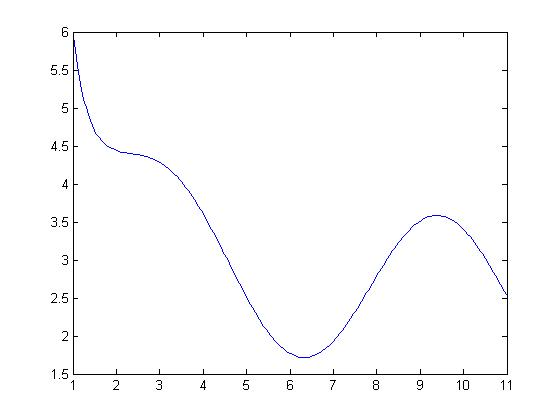
\includegraphics[width=10cm]{eval_1.jpg}
%\caption{plot of $y$ with no error}
%\label{eval_1}
%\end{figure}
%
%Then the evaluation of $Q(x)$ is shown in figure~\ref{eval_2}
%\begin{figure}[!htb]
%\centering
%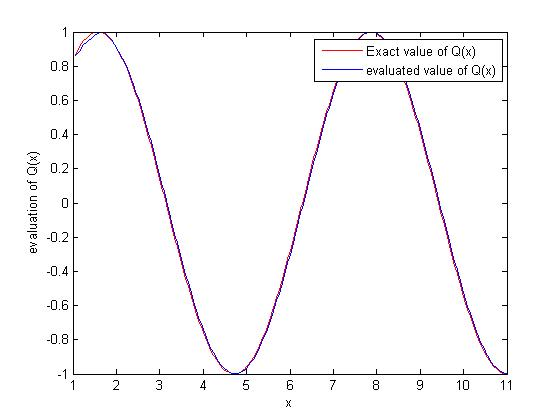
\includegraphics[width=10cm]{eval_2.jpg}
%\caption{ploy of $Q(x)$}
%\label{eval_2}
%\end{figure}
%
%Also,to determine the error, we calculate the SSE:
%\begin{verbatim}
%SSE =
%    0.0632
%\end{verbatim}
%
%For 200 points, SSE=0.0632 can meet our requirement of precision.

\subsection{Given Q(x), Find P(x),and without Input Errors}

Similarly, we suppose $e^{\int P \left( x \right) \tmop{dx}} = m \left( x
\right)$,and also get
\begin{equation}
  m \left( x \right) y \left( x \right) = \int_{x_0}^x m \left( x \right) Q
  \left( x \right) \tmop{dx}
\end{equation}
However,This is no longer {\tmstrong{Volterra Integral Equations of the First
Kind}},and it's the second kind of VIEs.

Let
\begin{eqnarray}
  \hat{Q} \left( x, x_i \right) & = & \left\{ \begin{array}{l}
    Q \left( x \right) \\
    0
  \end{array} \right. \begin{array}{c}
    x \leqslant x_i\\
    x > x_i
  \end{array}
\end{eqnarray}
Hence,we can get a well-posed second kind Fredholm Integral Equations.


\begin{equation}
  m \left( x_i \right) y \left( x_i \right) = \int_{x_0}^{x_n} m \left( x
  \right) \hat{Q} \left(x_j,x_i \right) d x
\end{equation}
we use quadrature methods to discretize above system,
\begin{equation}
  m \left( x_i \right) y \left( x_i \right) = \sum^n_{j = 1} \hat{Q} \left(
  x_j, x_i \right) m \left( x_j \right) \Delta x, i = 1, 2, \ldots, n
\end{equation}
i.e.
\begin{equation}
  \frac{1}{\Delta x} m \left( x_i \right) = \sum^n_{j = 1} \frac{\hat{Q}
  \left( x_j, x_i \right)}{y \left( x_i \right)} m \left( x_j \right), i = 1,
  2, \ldots, n
\end{equation}
Let $\frac{\hat{Q} \left( x_j, x_i \right)}{y \left( x_i \right)} = G_{i,
j}$,then we have
\begin{equation}
  G m = \frac{1}{\Delta x} m
\end{equation}
From above equation,we get $m$ is an eigenvector with eigenvalue
$\frac{1}{\Delta x}$ of $G$.

Sadly,it's easy to know that there $n$ different eigenvalues of G,if $Q (x_i)$
are different.Then,we will get n solutions.It's seemed that the question is
ill-posed as we have done above,but actualy,we only get one solution if we fix
$\Delta x$.

However,$\Delta x$ is certained,if we get $(x_i, y_i)$. So we should discuss
separately by the Value of $\Delta x$.
\begin{itemizedot}
  \item if $\frac{1}{\Delta x }$ is one of the eigenvalues of G,then we
  can calculate m by it.

  \item if $\frac{1}{\Delta x}$ is not one of the eigenvalue of G,which is
  more common.First of all, we choose most closed one $Q_i$(In fact, we can
  find that every $Q_i$ is one of the eigenvalues of $G$),that satisfying
  \begin{equation}
    \min_{i = \left\{ 1, 2, \ldots, n \right\}} \left( \frac{1}{\Delta x} -
    Q_i \right) \assign \alpha
  \end{equation}
  Now we solve equation
  \begin{equation}
    \left( G + \alpha I \right) m = \frac{1}{\Delta x} m
  \end{equation}
  We can solve it ,and get an $m_{\alpha}$ which is most closed solution.


\end{itemizedot}


\subsection{Given P(x), Find Q(x),and Have Input Errors}

Similarly with none errors case,we will get
\begin{equation}
  y^{\delta} \left( x_i \right) = \sum^n_{j = 1} \frac{\hat{m} \left( x_j, x_i
  \right) \Delta x}{m \left( x_i \right)} Q \left( x_j \right)
\end{equation}
thus we have $G_{i, j} = \frac{\hat{m} \left( x_j, x_i \right) \Delta x}{m
\left( x_i \right)}$,and we have a new form
\begin{equation}
  y^{\delta} = G Q
\end{equation}
by Tikhonov Regularization,we have minimum norm solution
\begin{equation}
  Q^{\delta}_{\alpha} = \left( G^{\ast} G + \alpha^2 I^{} \right)^{- 1}
  G^{\ast} y^{\delta}
\end{equation}


by Arcangeli Criterien,we choose
\begin{eqnarray}
  \alpha & = & \frac{\left\| G Q_{\alpha}^{\delta} - y^{\delta}
  \right\|}{\delta} \\
  & = & \frac{\left\| G \left( G^{\ast} G + \alpha^2 I^{} \right)^{- 1}
  G^{\ast} y^{\delta} - y^{\delta} \right\|}{\delta}
\end{eqnarray}


\subsection{Given Q(x), Find P(x),and Have Input Errors}

Similarly with none errors case,we will get
\begin{equation}
  y^{\delta} \left( x_i \right) m^{\delta} \left( x_i \right) = \sum^n_{j = 1}
  \hat{Q} \left( x_j, x_i \right) m^{\delta} \left( x_j \right) \Delta x, i =
  1, 2, \ldots, n
\end{equation}
\begin{equation}
  y^{\delta} \left( x_{} \right) m^{\delta} \left( x_{} \right) =
  \left(\begin{array}{c}
    \sum^n_{j = 1} \hat{Q} \left( x_j, x_1 \right) m^{\delta} \left( x_j
    \right) \Delta x\\
    \ldots\\
    \ldots\\
    \sum^n_{j = 1} \hat{Q} \left( x_j, x_n \right) m^{\delta} \left( x_j
    \right) \Delta x
  \end{array}\right)
\end{equation}
Suppose there is no errors in data $y$,then $y^{\delta} \left( x \right) = y
\left( x \right)$,by none error case,we have get a solution $m \left( x
\right)$,which also satisfying
\begin{equation}
  y^{} \left( x_{} \right) m \left( x_{} \right) = \left(\begin{array}{c}
    \sum^n_{j = 1} \hat{Q} \left( x_j, x_1 \right) m^{} \left( x_j \right)
    \Delta x\\
    \ldots\\
    \ldots\\
    \sum^n_{j = 1} \hat{Q} \left( x_j, x_n \right) m^{} \left( x_j \right)
    \Delta x
  \end{array}\right)
\end{equation}
Make $\tmop{substract}$ion between (59)\&(58),then we get
\begin{equation}
  y^{\delta} \left( x_{} \right) \left( m \left( x \right) - m^{\delta} \left(
  x \right) \right) = \left(\begin{array}{c}
    \sum^n_{j = 1} \hat{Q} \left( x_j, x_1 \right) \left( m \left( x_j \right)
    - m^{\delta} \left( x_j \right) \right) \Delta x\\
    \ldots\\
    \ldots\\
    \sum^n_{j = 1} \hat{Q} \left( x_j, x_n \right) \left( m \left( x_j \right)
    - m^{\delta} \left( x_j \right) \right) \Delta x
  \end{array}\right)
\end{equation}
Let $k \left( x \right) = m \left( x \right) - m^{\delta} \left( x
\right)$,then $k (x)$ also fixes equation (59) (changes m into k).We have
claims that if $\Delta x$ is stable,then we can only find one solution. Thus
we cannot find another $m (x)$ if we suppose $y^{\delta} \left( x \right) = y
\left( x \right)$.i.e $m \left( x \right) = m^{\delta} \left( x \right)$,or $m
\left( x \right) =\tmmathbf{0}$.

From above discussion,we know that if we do not make a regularization of this
second kind of Fredholm equation, we won't clean away or even decrease the
data errors.
\newpage
\section{\textsc{MatLab} interpolation approach to specific parameter estimation problems}
\subsection{Constant Parameter Scenario: Multiple Shooting method}


We can see that it is not easy to estimate our parameter $p(x)$ and $q(x)$ in our first order linear equation. However, if the form of $p(x)$ and $q(x)$ are given, like $\sin \alpha x$, in which $\alpha$ is to be determined, then we can use \textsc{MatLab} to accomplish this mission. In addition, if we only need to consider one parameter, say $\alpha$ in $\sin \alpha x$, then we even can endure some error since we will use least square method.
In \textsc{MatLab}, we will use function \verb$fminsearch$ to determine our goal function SSE (Sum-Square-of-errors)
To visualize our task, we can now assume that our differential equation is:

\begin{equation}
\frac{\text{d}y}{\text{d}t}=\sin \alpha t+\cos \beta y
\end{equation}


First, we should produce a series of accurate data, and plus our noise in it for the second case. We assume that our noise, which is a Random Variable, satisfy $noise\sim N(0,{{0.01}^{2}})$ (Gaussian White Noise) .In \textsc{MatLab} it can be expressed as :
\begin{verbatim}
noise=normrnd(MU,SIGMA,m,n)
\end{verbatim}
where m,n is the size of matrix. We first solve our problem assuming that our observation data is with no noise.

\subsubsection{No Noise applied}

Now we produce our accurate data, which will be used as our observed data.\\
1.determine our dy fuction (destination.m)
\begin{verbatim}
function dy = destination(t,y,flag,alpha,beta)
dy=sin(alpha*t)+cos(beta*y);
\end{verbatim}
2.use ODE45 to solve the equation and plot the accurate data(command line)
\begin{verbatim}
y0=3;alpha=4;beta=5;N=1000;
tspan=linspace(0,10,N);
[t ymodelt]=ode45('destination',tspan,y0,[],alpha,beta);
[t ymodel]=ode45('destination',tspan,y0,[],alpha,beta);
plot(t,ymodel);
\end{verbatim}

Fig 4.1

3.In order to solve for alpha, beta using \verb$fminsearch$, we need to write a function which can calculate the error of our estimation and the data given above. Let’s call such function SSE\_1.m(Sum-Square-of-errors)
\begin{verbatim}
function val=SSE_1(k,tspan,yobs)
alpha=k(1);
beta=k(2);
tspan=tspan';
y0=3;
[t ymodel]=ode45('destination',tspan,y0,[],alpha,beta);
resid=ymodel-yobs;
val=resid'*resid;
\end{verbatim}

4.We can now plot alpha-beta-SSE plot simply using SSE\_1:
\begin{verbatim}
x=2:0.1:6;
y=2:0.1:6;
[X Y]=meshgrid(x,y);
for m=1:41
    for n=1:41
        Z(m,n)= SSE_1([X(m,n) Y(m,n)],tspan, ymodelt);
    end
end
grid on;
surf(X,Y,Z);
shading interp;
xlabel('alpha');ylabel('beta'); zlabel('SSE');
view([60 50]);
\end{verbatim}


\begin{figure}[H]
\centering
\subfigure[ SSE plot]{
\label{SSE_1-1}
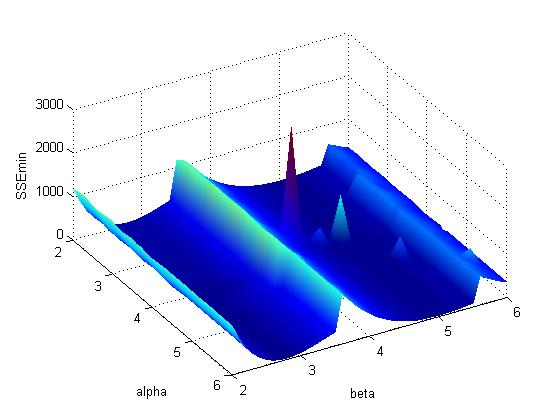
\includegraphics[width=12cm]{SSE_1-1.jpg}}
\subfigure[ SSE plot ($\alpha$)]{
\label{SSE_1-2}
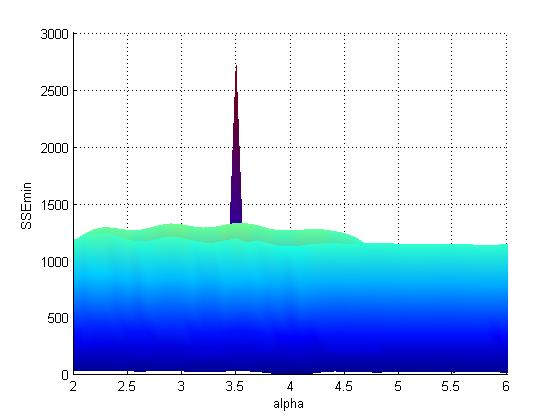
\includegraphics[width=7.3cm]{SSE_1-2.jpg}}
\subfigure[SSE plot ($\beta$)]{
\label{SSE_1-3}
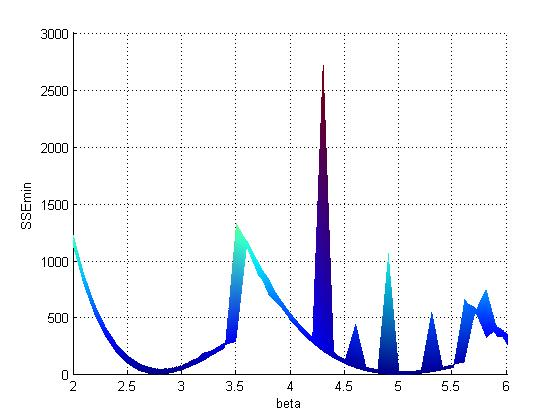
\includegraphics[width=7.3cm]{SSE_1-3.jpg}}
\caption{SSE plot respect to $\alpha$ and $\beta$}
%\label{Fig.lable}
\end{figure}

We can clearly see that when $\alpha \approx 4$ and $\beta \approx 2.8$ and $4.9$ the SSE gets its minimum. For more precise calculation, we should use \verb$fminsearch$ to get $\alpha$ and $\beta$.
Recall that we now have \verb$tspan$, \verb$ymodelt$ and we should give \textsc{MatLab} initial estimation of alpha and beta. Then we can use \verb$fminsearch$ to directly solve the problem. We shall now guess that $\alpha=4$ and $\beta=2.8$:
\begin{verbatim}
>> k=[4 2.8];
>> [k SSEmin]=fminsearch('SSE_1',k,[],tspan,ymodelt)
\end{verbatim}
The result is:
\begin{verbatim}
k =
    4.0426    2.7839
SSEmin =
1.5513
>> k=[4.0426 2.7839];
>> [k SSEmin]=fminsearch('SSE_1',k,[],tspan,ymodelt)
k =
    4.0426    2.7838
SSEmin =
    1.5513
\end{verbatim}
The process of iteration indicate that point \verb$[4.0426 2.7839]$ is really the local minimum.
Don’t forget that we have another approximation $\alpha=4$ and $\beta=4.9$:
\begin{verbatim}
>> k=[4 4.9]
>> for m=1:6
[k SSEmin]=fminsearch('SSE_1',k,[],tspan,ymodelt);
	k
	SSEmin
end

k =
    4.0001    4.9988
SSEmin =
   5.8807e-04
k =
    4.0004    5.0002
SSEmin =
   1.6218e-04
k =
    4.0004    5.0002
SSEmin =
   1.5774e-04
\end{verbatim}
Such iteration indicates that \verb$k=[4.0004 5.0002]$ is the final answer given by \textsc{MatLab}. We now compare the SSE of two local minimum: \verb$1.5774e-04$ when \verb$k=[4.0004 5.0002]$ and 1.5513 when \verb$k=[4.0426 2.7839]$. It is obvious that we should choose \verb$k=[4.0004 5.0002]$, which means that the approximation for $\alpha$ and $\beta$ using numerical method is given by $\alpha=4.0004$ and $\beta=5.0002$, which indeed close to the exact value $\alpha=4.0000$ and $\beta=5.0000$.



\subsubsection{Noise applied}

We shall now consider the case that the observed data is with noise. To see whether noise is actually distributed as normal distribution, we call draw a graph:
\begin{verbatim}
noise=normrnd(0,0.01,1000,1);
[a,b]=hist(noise);
bar(b,a/sum(a))
\end{verbatim}

\begin{figure}[htb]
\centering
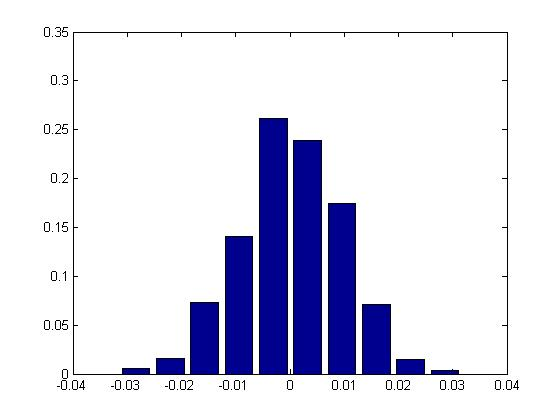
\includegraphics[width=10cm]{4-0.jpg}
\caption{Distribution of noise}
\label{4-0}
\end{figure}

1.add our noise and plot the data again in Figure~\ref{4-2} \ and Figure~\ref{4-3}
\begin{verbatim}
for i=1:1000
    ymodelt(i)=ymodelt(i)+noise(i);
end
plot(t,ymodelt);
hold on;
plot(t,ymodel,'r');
xlabel('t');ylabel('y');
hold off;
\end{verbatim}

\begin{figure}[H]
\centering
\subfigure[Observed Data]{
\label{4-2}
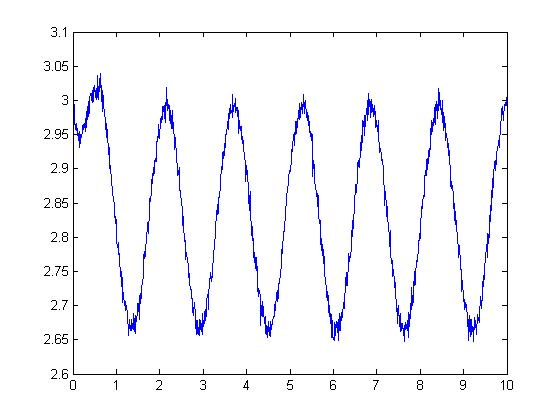
\includegraphics[width=7.3cm]{4-2.jpg}}
\subfigure[Comparison of data with and without noise]{
\label{4-3}
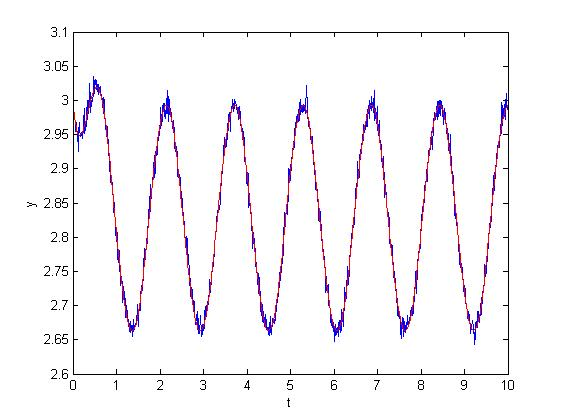
\includegraphics[width=7.3cm]{4-3.jpg}}
\caption{Data with noise}
%\label{Fig.lable}
\end{figure}


2.We shall first eliminate our noise in order to process our data using FFT (Fast Fourier Transformation)(Figure~\ref{4-4}) and IFFT (Inverse Fast Fourier Transform). After FFT and IFFT, the magnitude of our data will shrink, so we should amplify our data.
\begin{verbatim}
z= fft(ymodelt);%FFT
po=1:1:1000;
plot(po,z);
xlabel('relative frequency');ylabel('amplitute');
\end{verbatim}

\begin{figure}[!htb]
\centering
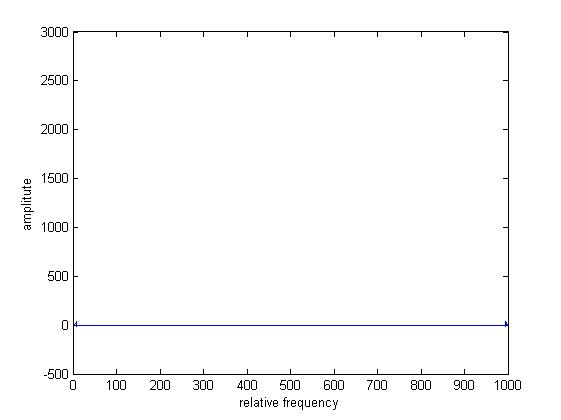
\includegraphics[width=10cm]{4-4.jpg}
\caption{FFT of Observed Data}
\label{4-4}
\end{figure}

3.We can see that we should eliminate the high frequency part and do the IFFT. Note that in the Figure below, the red plot is our data after IFFT and the green plot is our origin data.
\begin{verbatim}
filter(1:50)= 1;%filter magnitude
filter(51:N)=0.00;%
for i=1:N
    thispy(i)= filter(i)*z(i);%filter
end
Z=ifft(thispy,N);%IFFT
plot(t,Z, 'r-');
hold on;
plot(t,ymodelt, 'g-');
\end{verbatim}

\begin{figure}[!htb]
\centering
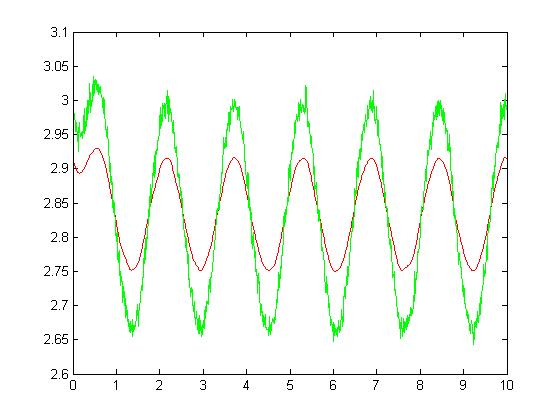
\includegraphics[width=7.3cm]{4-5.jpg}
\caption{Data After FFT and IFFT}
\label{4-5}
\end{figure}

4.Amplification of our data:
\begin{verbatim}
Z=abs(Z);%eliminate imaginary number
ymodel_average = sum(ymodel)/length(ymodel);
Z_average = sum(Z)/length(Z);
averageDelta = ymodel_average - Z_average;
ymodel_max=max(ymodel);
ymodel_min=min(ymodel);
for i=1:N
    Z(i)=Z(i)+ averageDelta;%move Z in order to meet the average of original data
end
Z_max=max(Z);
Z_min=min(Z);
Amplify=min((ymodel_max- ymodel_average)/( Z_max -  ymodel_average), (ymodel_min-
ymodel_average)/( Z_min -  ymodel_average));
for i = 1 : N
    Z(i)= ymodel_average+(Z(i)- ymodel_average)* Amplify;
end
plot(t, Z);
hold off;
\end{verbatim}

\begin{figure}[!htb]
\centering
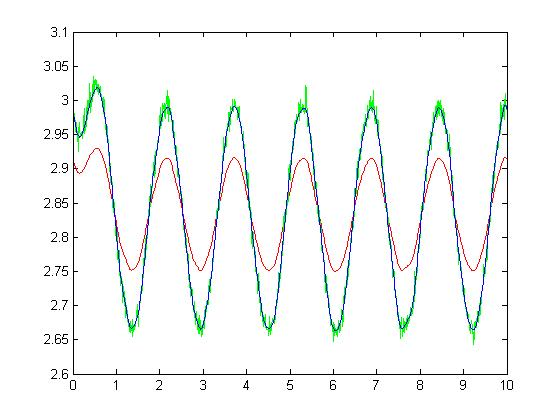
\includegraphics[width=10cm]{4-6.jpg}
\caption{Data after amplification (Blue)}
\label{4-6}
\end{figure}

5.We can see that our data’s noise is virtually eliminated. After this procedure, the process of getting SSE is the same.
\begin{verbatim}
ymodelt=Z';
clear Z;
x=2:0.1:6;
y=2:0.1:6;
[X Y]=meshgrid(x,y);
for m=1:41
    for n=1:41
        Z(m,n)= SSE_1([X(m,n) Y(m,n)],tspan, ymodelt);
    end
end
grid on;
surf(X,Y,Z);
shading interp;
xlabel('alpha');ylabel('beta'); zlabel('SSE');
view([60 50]);
\end{verbatim}

\begin{figure}[htb]
\centering
\subfigure[ SSE plot]{
\label{SSE_1-4}
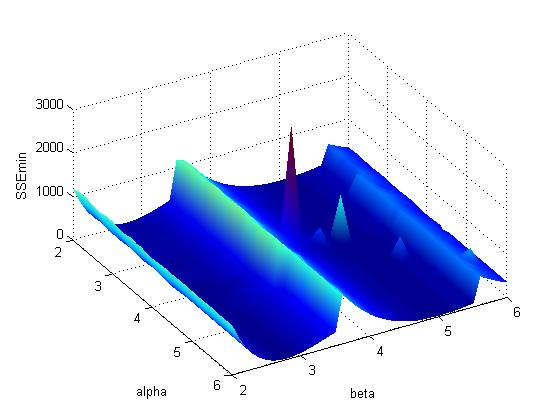
\includegraphics[width=12cm]{SSE_1-4.jpg}}
\subfigure[ SSE plot ($\alpha$)]{
\label{SSE_1-5}
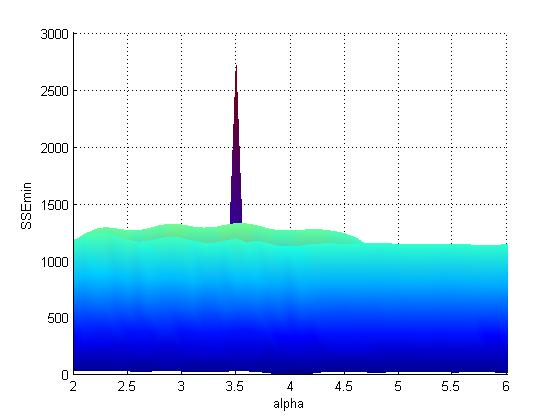
\includegraphics[width=7.3cm]{SSE_1-5.jpg}}
\subfigure[SSE plot ($\beta$)]{
\label{SSE_1-6}
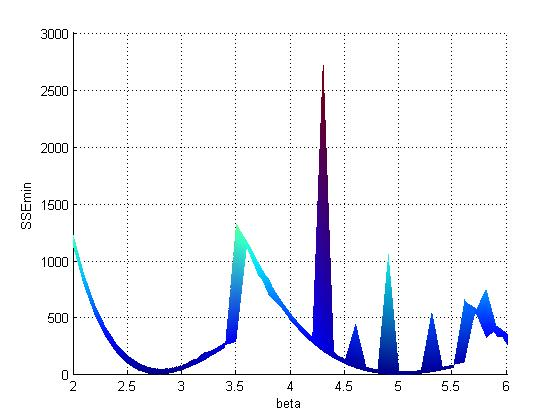
\includegraphics[width=7.3cm]{SSE_1-6.jpg}}
\caption{SSE plot respect to $\alpha$ and $\beta$}
\label{SSE_1-4,5,6}
\end{figure}

6.It is not astonishing that the SSE figures (Figure~\ref{SSE_1-4,5,6}) before and after the noise is added are nearly the same. Such result indicates that FFT and IFFT really work in this scenario. And what we should do now is merely repeat fminsearch to get the best approximation of $\alpha$ and $\beta$
\begin{verbatim}
>> k=[4 2.8];
>> for m=1:2
    [k SSEmin]=fminsearch('SSE_1',k,[],tspan,ymodelt);
    k
    SSEmin
end
k =
    4.0450    2.7829
SSEmin =
    1.7462
k =
    4.0450    2.7829
SSEmin =
    1.7462

>> k=[4 4.9];
>> for m=1:6
    [k SSEmin]=fminsearch('SSE_1',k,[],tspan,ymodelt);
    k
    SSEmin
end
k =
    4.0001    4.9988
SSEmin =
    0.0181
k =
    4.0001    4.9988
SSEmin =
    0.0181
k =
    4.0001    4.9987
SSEmin =
    0.0178
k =
    4.0001    4.9987
SSEmin =
    0.0178
\end{verbatim}
Under the initial condition $\alpha=4,\beta=2.8$ and $\alpha=4,\beta=4.9$, the result of iteration using \verb$fminsearch$ indicates that the best approximation of $\alpha$ and $\beta$ is $\alpha=4.0001,\beta=4.9987$

\subsubsection{Conclusion}
We now conclude our answer:


\begin{table}[htbp]
\label{34}
\centering
\caption{Conclusion of $\alpha$ and $\beta$}
\begin{tabular}{lcc}
\toprule
              &  $\alpha$ &   $\beta$ \\
\midrule
exact value   &   4.0000  &    5.0000 \\
without noise &   4.0004  &    5.0002 \\
with noise    &   4.0001  &    4.9987 \\
\bottomrule
\end{tabular}
\end{table}

Such approximation can meet our precision.\\
\section{Interpolation Methods}
suppose we have several points given by the coordinate: $(x_{1},y_{1});(x_{2},y_{2});(x_{3},y_{3})........(x_{n},y_{n})$. given $x\in[x_{j-1},x_{j}]$,how to get the y value corresponding to x ?we can use some functions called interpolate to estimate the y value, and this method is called interpolation.
\subsection{Linear Interpolation}
this method creates linear function connecting two points $(x_{j-1},y_{j-1});
 (x_{j},y_{j})$
  $$y=y_{j-1}+\frac{(x-x_{j-1})(y_{j}-y_{j-1})}{(x_{j}-x_{j-1})}$$
for any $x$ in between, we can get corresponding y through this linear function.
\subsection{Polynomial Interpolation}
assume we have n points, there exists unique nth order polynomial that can connect these n points, this nth order polynomial is called Polynomial interpolate .
\par
Lagrange polynomial (one method to get this n
 th order polynomial):

$$P(x)=\sum_{j=1}^{n}\prod_{i=1,i\neq j}^{n}\frac{x-x_{j}}{x_{i}-x_{j}}y_{i}$$
\subsection{Cubic Spline Interpolation}
Basically, for each two successive points, spline is a local 3rd order polynomial crossing these points. But we have an additional requirement, that is the 1st and 2nd derivative must be continuous especially at every boundary point.
\par

Assume we have n+1 points,$(x_{0},y_{0}); (x_{1},y_{1})  ;(x_{2},y_{2}); (x_{3},y_{3}),...,(x_{n},y_{n})$. Let $S_{i}(x)$ be the cubic spline function between $[x_{i},x_{i+1})(i=0,1,2,3.....,n-1)$. let $$S_{i}(x)=a_{i}x^{3}+b_{i}x^{2}+c_{i}x+d_{i}$$
where a,b,c,d are unknown parameters. in summery we have 4n unknown parameters , by common sense we need 4n linear equations.
\par
Since for $\forall S_{i}(x),S(x_{i})=y_{i},S(x_{i+1})=y_{i+1}$
  we can get 2n linear equations,

$\forall x_{i}
  S_{i-1}^{'}(x_{i})=S_{i}^{'}(x_{i})i=1,2,3,....,n-1$
  we get another n-1 linear equations.

$\forall x_{i}
  S_{i-1}^{''}(x_{i})=S_{i}^{''}(x_{i}),i=1,2,3,....,n-1$
 we get another n-1 linear equations.
\par
In summary we have 4n-2 equations, so we can have two dimension of freedom. the normal process is setting $S_{0}^{''}(x_{0})=0,S_{n-1}^{''}(x_{n-1})=0$
 ,such that we eliminate the rest dimension of freedom.
\par
finally, in order to get these 4n unknown parameters. our task become to solve n-1 linear equations, that is to solve the reverse of$(n-1)\times(n-1)$matrix.
\subsection{Other Interpolation Methods}
\subsubsection{Rational Functions}
this method use the rational function to estimate values.
\subsubsection{Trigonometric Interpolation}
this method use trigonometric-sum to approximate discrete data. explicitly, the function should be $$f(x)=a_{0}+\sum_{n=1}^{N}a_{n}cos(nx)+\sum_{n=1}^{N}b_{n}sin(nx)$$


\section{$P(x)$ Estimation by Using \textsc{MatLab} Interpolation Method}


Interpolation is a method of constructing new data points within the range of a discrete set of known data points.
In engineering and science, one often has a number of data points, obtained by sampling or experimentation, which represent the values of a function for a limited number of values of the independent variable. It is often required to interpolate (i.e. estimate) the value of that function for an intermediate value of the independent variable. This may be achieved by curve fitting or regression analysis.\\
In our case, we using interpolation to accomplish the parameter estimation problem of differential equation which has the form:
\begin{equation}
\frac{{dy}}{{dx}} = P(x)y + Q(x)
\end{equation}

and during the process, a comparison between different \textsc{MatLab} interpolation methods is also shown in the paper.

\subsection{Continue $P(x)$ fitting}
\subsubsection{A special case study: $Q(x)=0$}
Let's begin with P(x) which is continuous, and we shall first discuss a special case that $Q(x)=0$.\\
Now we produce our accurate data, which will be used as our observed data.\\
1.determine our P(x) function (expinter.m)
\begin{verbatim}
x=0.1:0.05:7;
y=exp(-cos(x));
\end{verbatim}
2.use spline function to interpolate the original data into a more accurate one
\begin{verbatim}
xi=0.1:0.01:7;                        %细化插值变量
yi=interp1(x,y,xi,'spline');                 %调用spline插值法求得数组yi
\end{verbatim}
3.In order to solve for $P(x)$, the value of $\frac{{dy}}{{dx}}$ is obviously necessary. Here we have two ways to go, one is to get the value of $\frac{{dy}}{{dx}}$ every five points (expinter.m), and we need to do interpolation again to get a more accurate data of P(x), while the other one only needs to have one interpolation because it get value of $\frac{{dy}}{{dx}}$ every point (expintercubic.m). It is easy for us to give an assumption that the second method is better than the first one, and we shall use $P(x) = \cos x$ as an example to verify this.\\
The first method:
\begin{verbatim}
for k=1:(length(y)-1)
    dyi(k)=(yi(5*k)-yi(5*k-1))/(xi(5*k)-xi(5*k-1));
    p(k)=dyi(k)/y(k+1);
end
    x2=0.15:0.05:7;
    x3=0.15:0.01:7;
    pnew=interp1(x2,p,x3,'spline');
    plot(x3,sin(x3),'k.',x3,pnew,'r')
    title('Method1','fontweight','bold')
    xlabel('x','fontsize',10)
    ylabel('p(x) fitting','fontsize',10)
    legend('y=sin(x)','P(x) fitting plot')
    grid on;
    sigma=0;
for t=1:length(x3)
        sigma=sigma+(pnew(t)-sin(x3(t)))^2;
end
    sigma
\end{verbatim}
The second method:
\begin{verbatim}
for k=1:(length(yi)-1)
    dyi(k)=(yi(k+1)-yi(k))/(xi(k+1)-xi(k));
    p(k)=dyi(k)/yi(k+1);
end
    x3=0.11:0.01:7;
    plot(x3,sin(x3),'k.',x3,p,'r')
    title('Method2','fontweight','bold')
    xlabel('x','fontsize',10)
    ylabel('p(x) fitting','fontsize',10)
    legend('y=sin(x)','P(x) fitting plot')
    grid on;
    sigma=0;
for t=1:length(x3)
        sigma=sigma+(p(t)-sin(x3(t)))^2;
end
    sigma
\end{verbatim}
Notice that all of the interpolation methods we used in these two methods are \verb$spline$, which ensures the reliability of this comparison.
\begin{figure}[H]
\subfigure[Method 1]{
\label{1_1}
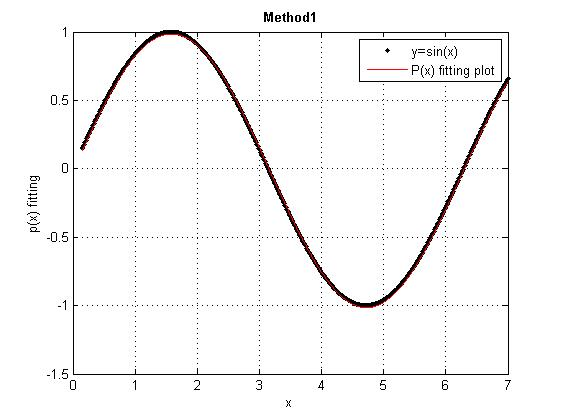
\includegraphics[width=7.3cm]{method1.jpg}}
\subfigure[Method 2]{
\label{1_2}
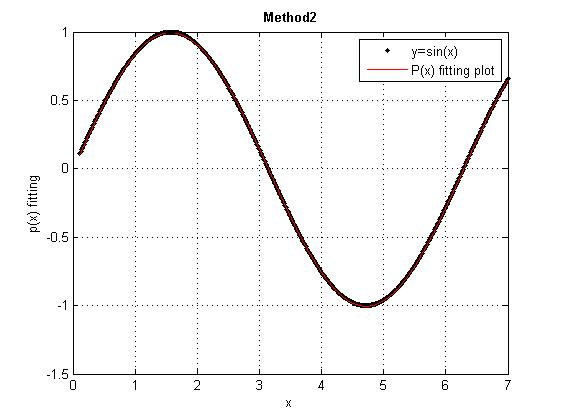
\includegraphics[width=7.3cm]{method2.jpg}}
\caption{The fitting plot of Method1 and Method2}
%\label{Fig.lable}
\end{figure}

And the result of sigma(SSE: sum square of the error) is:
\begin{verbatim}
>> expinter
sigma =
    0.1390
>> expintercubic
sigma =
    0.0156
\end{verbatim}

Obviously, the SSE of the second method is much smaller than the first one, and this is easy to understand because every time you do an interpolation, new error would be made and at last they would composite and become an even larger error.\\
\subsubsection{\textsc{MatLab} interpolation methods' study when $Q(x)=0$}
So based on the second method, we shall do a comparison between different \textsc{MatLab} interpolation method:
1.\verb$linear$ interpolation\\
Linear interpolation is a method of curve fitting using linear polynomials. It is quick and easy, but it is not very precise. Another disadvantage is that the interpolant is not differentiable at the point ${x_k}$. As we shall see, its SSE is much bigger than the other methods'.
\begin{verbatim}
yi=interp1(x,y,xi,'linear');                 %调用linear插值法求得数组yi
\end{verbatim}
2.\verb$spline$ interpolation\\
Spline interpolation uses low-degree polynomials in each of the intervals, and chooses the polynomial pieces such that they fit smoothly together. The resulting function is called a spline. And compare with linear interpolation, spline interpolation has a smaller error and the interpolant is smoother.
\begin{verbatim}
yi=interp1(x,y,xi,'spline');                 %调用spline插值法求得数组yi
\end{verbatim}
3.\verb$cubic$ interpolation\\
In the mathematical subfield of numerical analysis a cubic Hermite spline (also called cspline), named after Charles Hermite, is a third-degree spline with each polynomial of the spline in Hermite form. The Hermite form consists of two control points and two control tangents for each polynomial. We shall see in the later result, because the Hermite polynomials it use is third-degree, of which the degree is same as \verb$spline$ function, the SSE of these two methods have little difference.
\begin{verbatim}
yi=interp1(x,y,xi,'cubic');                 %调用cubic插值法求得数组yi
\end{verbatim}
The \textsc{MatLab} plots here:

\begin{figure}[H]
\centering
\subfigure[Linear interpolation]{
\label{inter1_1}
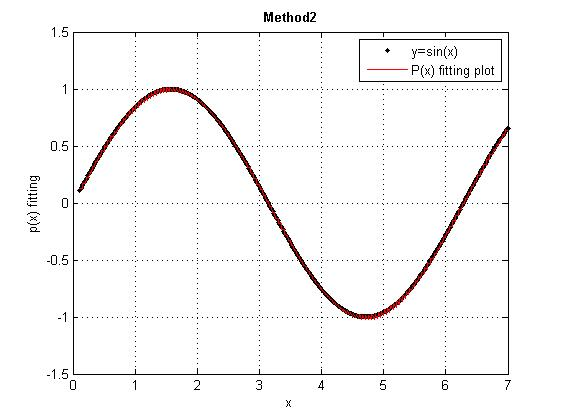
\includegraphics[width=7.3cm]{linear.jpg}}
\subfigure[Spline interpolation]{
\label{inter1_2}
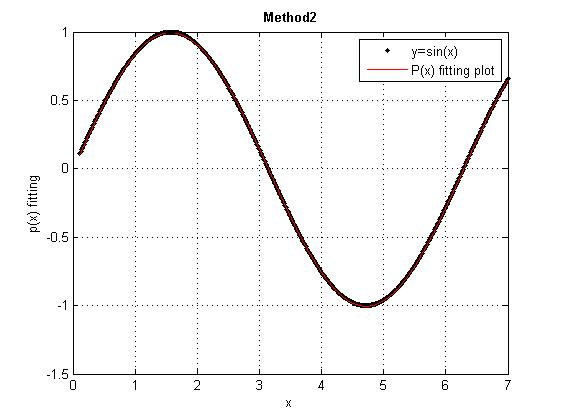
\includegraphics[width=7.3cm]{spline.jpg}}
\subfigure[Cubic interpolation]{
\label{inter1_3}
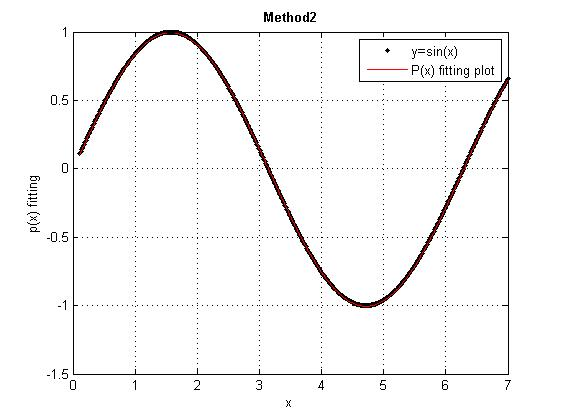
\includegraphics[width=7.3cm]{cubic.jpg}}
\caption{Fitting plot of the three methods}
%\label{Fig.lable}
\end{figure}
And the SSE of these methods are:\\
1.\verb$linear$ interpolation:
\begin{verbatim}
sigma =
    0.1399
\end{verbatim}
2.\verb$spline$ interpolation:
\begin{verbatim}
sigma =
    0.0156
\end{verbatim}
3.\verb$cubic$ interpolation:
\begin{verbatim}
sigma =
    0.0173
\end{verbatim}
As we see, just like what we assume before, \verb$linear$ interpolation has the biggest SSE while \verb$spline$ interpolation and \verb$cubic$ interpolation have smaller ones and the difference of them is little.(The more detailed analysis of their accuracy level will be shown in the theoretical analysis part of these interpolation method.)
\subsubsection{General case: when $Q(x) \ne 0$}
However, here we still need to have the condition that $Q(x)$ is known. For such case it is easy to understand that the question is still easy, because we just need to minus the value of $Q(x)$ from $\frac{{dy}}{{dx}}$, divide the value of $y$, and then we would get the $P(x)$ at that point. This is almost the same as the case when $Q(x)=0$, so we would not give an example.
\subsection{Discontinue $P(x)$ fitting}
For convenience, we assume $Q(x)=0$
Now we produce our accurate data, which will be used as our observed data.\\
1.determine our P(x) function (uncontinue.m)
\begin{verbatim}
x=-1:0.05:3;
x01=-1:0.05:1;
y01=exp(0.5*x01.^2);
x02=1.05:0.05:3;
y02=exp(-0.5*x02.^2+1);
y=[y01,y02];
\end{verbatim}
Which means that $P(x)=x$ on $[-1,1]$ and $P(x)=-x$ on $(1,3]$.\\
2.use spline function to interpolate the original data into a more accurate one
\begin{verbatim}
xi=-1:0.01:3;                        %细化插值变量
yi=interp1(x,y,xi,'spline');                 %调用spline插值法求得数组yi
\end{verbatim}
3.Like before, we need to get the value of $\frac{{dy}}{{dx}}$ to solve for $P(x)$, and then plot it out and calculate its SSE. Here the interpolation method we use is \verb$spline$ function.\\
Solve for $P(x)$:
\begin{verbatim}
for k=1:(length(yi)-1)
    dyi(k)=(yi(k+1)-yi(k))/(xi(k+1)-xi(k));
    p(k)=dyi(k)/yi(k+1);
end
\end{verbatim}
Plot it out:
\begin{verbatim}
    x3=-0.99:0.01:3;
    x4=-0.99:0.01:1;
    x5=1:0.01:3;
    subplot(1,2,1),plot(x3,p,'r.')
    title('Spline fitting of p(x)','fontweight','bold')
    xlabel('x','fontsize',10)
    ylabel('p(x) fitting','fontsize',10);
    subplot(1,2,2),plot(x4,x4,'k',x5,-x5,'k')
    title('Real p(x)','fontweight','bold')
    xlabel('x','fontsize',10)
    ylabel('p(x)','fontsize',10);
\end{verbatim}
Solve for SSE:
\begin{verbatim}
    sigma=0;
for t=1:(length(x4)-1)
    sigma=sigma+(p(t)-x4(t))^2;
end
for t=1:length(x5)
    sigma=sigma+(p(t+length(x4)-1)+x5(t))^2;
end
    sigma
\end{verbatim}
And the fitting plot is:
\begin{figure}[!htb]
\centering
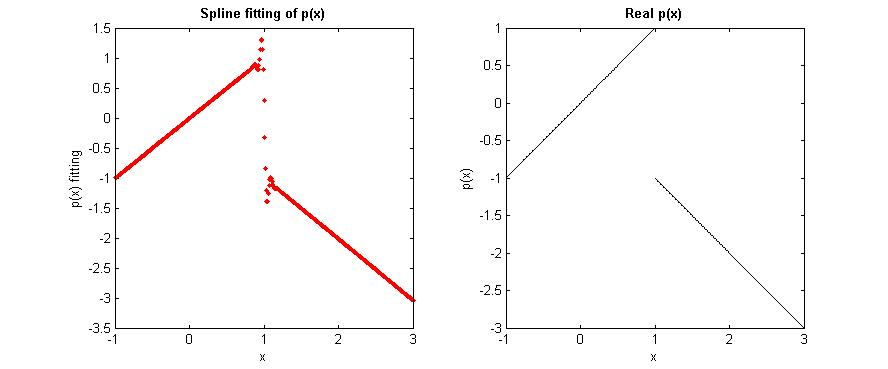
\includegraphics[width=16.6cm]{discontinue.jpg}
\caption{Fitting P(x) and the original P(x)}
\label{dis1_1}
\end{figure}
And the result of SSE is:
\begin{verbatim}
>> uncontinue
sigma =
    2.9607
\end{verbatim}
From the picture, one can easily figure out the discontinuity of $P(x)$, and can easily told a small interval that the discontinue point in. And then we can divide the discussion of $P(x)$ into two parts, one is from the lower bound of the domain of definition to the discontinuous point, another is from the point to the upper bound, and that come backs to the case that $P(x)$ is continue. Also, it is easy to observe that the SSE here is a little bit large, however if we remove the 10 points around 1 when we are calculating the SSE, we shall see that it would become a very small value.\\
\begin{verbatim}
for t=1:(length(x4)-5)
    sigma=sigma+(p(t)-x4(t))^2;
end
for t=5:length(x5)
    sigma=sigma+(p(t+length(x4)-1)+x5(t))^2;
end
    sigma
\end{verbatim}
And the SSE become:
\begin{verbatim}
sigma =
    0.4658
\end{verbatim}
which is a quite small one. This shows that the fitting result is quite good at the two sides of the function.\\
So from all of the discussion, we need to conclude what we get:\\
1.How to use the \textsc{MatLab} interpolation method solving the problem of parameter estimation.(continue and discontinue)\\
2.Among all the interpolation method, \verb$linear$ function has the lowest accuracy level while \verb$spline$ function and \verb$cubic$ function are better.\\

\section{Conclusion and Distribution}
At the beginning of our article, we posted four questions, and three of them can be answer by such demonstration with \textsc{MatLab}. They are:
\par
1. How can we obtain parameters from such model (approximation)\\
Using least square criterion, we calculate the Sum-Square-of-errors (SSE) to obtain our parameter\
\par
2. Is the model existing the only one model (uniqueness)?\\
The answer to such question cannot completely answered by the example accompanied with \textsc{MatLab}. However, we can sure that there is situation where the parameter of our model is unique, it can be seen in the example ‘Constant Parameter Scenario’, where $\beta$ can be either 2.78 or 5.00 (approximation).
\par
3. Can the model endure little error of the output (stability)?\\
The answer is surely illustrated by example with \textsc{MatLab}. We can see that FFT and IFFT is a very useful tool to erase the noise. We pick a noise which is distributed as normal distribution, which simulate the actual scenario of measurement.\\

Distribution:\\
W. Zhang: Discritization,SVD ,Methods of Regularization,Iterative method,Applications of Regularization\\
Q. Wu: Multiple Shooting Method with \textsc{MatLab},SVD, redaction\\
J. Wang: $P(x)$ Estimation with \textsc{MatLab} (Cont. and DisCont. case)\\
T. Luo: Interpolation Methods\\

\begin{thebibliography}{11}
  \bibitem[1]{3}G.~Backus and F.~Gilbert.{\newblock} Uniqueness in the
  inversion of inaccurate gross earth data.{\newblock} \tmtextit{Philosophical
  Transactions for the Royal Society of London. Series A, Mathematical and
  Physical Sciences}, :123--192, 1970.{\newblock}

  \bibitem[2]{5}G.H.~Golub and C. F. Van~Loan.{\newblock} \tmtextit{Matrix
  Computation}.{\newblock} The Johns Hopkins University Press,
  1996.{\newblock}

  \bibitem[3]{6}Charles W.~Groetsch.{\newblock} \tmtextit{Inverse Problems in
  the Mathematical Sciences}.{\newblock} Informatica International, Inc.,
  1993.{\newblock}

  \bibitem[4]{7}And A. Neubauer~H.W.Engl, M.Hanke.{\newblock}
  \tmtextit{Regularization on Inverse Problem}.{\newblock} Kluwer Academic
  Publishers, 1996.{\newblock}

  \bibitem[5]{1}A.~Kirsch.{\newblock} \tmtextit{An introduction to the
  mathematical theory of inverse problems}, volume 120.{\newblock} Springer,
  2011.{\newblock}

  \bibitem[6]{4}C.~Lanczos.{\newblock} \tmtextit{Linear Differential
  Operators}.{\newblock} SIAM, 1996.{\newblock}

  \bibitem[7]{11}Vogel C~R.{\newblock} Non-convergence of the l-curve
  regularization parameter selection method.{\newblock} \tmtextit{Inverse
  Problems}, :535--547, 1996.{\newblock}

  \bibitem[8]{2}A.~Tarantola.{\newblock} \tmtextit{Inverse problem theory and
  methods for model parameter estimation}.{\newblock} Society for Industrial
  Mathematics, 2005.{\newblock}

  \bibitem[9]{10}Arsenin V Y~Tikhonov A N.{\newblock} \tmtextit{Solutions of
  Ill-Posed Problems}.{\newblock} John Wiley and Sons, 1977.{\newblock}

  \bibitem[10]{9}Groesch C~W.{\newblock} \tmtextit{The Theory of Tikhonov
  Regularization for Fredholm Equations of the First Kind}.{\newblock} Pitman
  Advanced Publishing Program, 1984.{\newblock}

  \bibitem[11]{IPMS}Groesch C~W.{\newblock} \tmtextit{Inverse Problems in the Mathematical Sciences}.{\newblock} vieweg Inc.{\newblock}

\end{thebibliography}



\end{document}
